%===============================================================================
% LaTeX sjabloon voor de bachelorproef toegepaste informatica aan HOGENT
% Meer info op https://github.com/HoGentTIN/latex-hogent-report
%===============================================================================

\documentclass[dutch,dit,thesis]{hogentreport}

% TODO:
% - If necessary, replace the option `dit`' with your own department!
%   Valid entries are dbo, dbt, dgz, dit, dlo, dog, dsa, soa
% - If you write your thesis in English (remark: only possible after getting
%   explicit approval!), remove the option "dutch," or replace with "english".

\usepackage{lipsum} % For blind text, can be removed after adding actual content

%% Pictures to include in the text can be put in the graphics/ folder
\graphicspath{{graphics/}}

%% For source code highlighting, requires pygments to be installed
%% Compile with the -shell-escape flag!
\usepackage[section]{minted}
\usepackage{mdframed}
\usepackage{amsmath}
%% If you compile with the make_thesis.{bat,sh} script, use the following
%% import instead:
%% \usepackage[section,outputdir=../output]{minted}
\usemintedstyle{solarized-light}
\definecolor{bg}{RGB}{253,246,227} %% Set the background color of the codeframe

%% Change this line to edit the line numbering style:
\renewcommand{\theFancyVerbLine}{\ttfamily\scriptsize\arabic{FancyVerbLine}}

%% Macro definition to load external java source files with \javacode{filename}:
\newmintedfile[javacode]{java}{
    bgcolor=bg,
    fontfamily=tt,
    linenos=true,
    numberblanklines=true,
    numbersep=5pt,
    gobble=0,
    framesep=2mm,
    funcnamehighlighting=true,
    tabsize=4,
    obeytabs=false,
    breaklines=true,
    mathescape=false
    samepage=false,
    showspaces=false,
    showtabs =false,
    texcl=false,
}

% Other packages not already included can be imported here

%%---------- Document metadata -------------------------------------------------
% TODO: Replace this with your own information
\author{Sebastiaan Delodder}
\supervisor{Mevr. S. Vandermeersch}
%\supervisor{Dhr. F. Van Houte}
%\cosupervisor{Mevr. S. Beeckman}
\title[]%
    {Optimalisatie van mobiele app performantie bij streaming-applicaties: React Native vs Ionic op het Android- platform.}
\academicyear{\advance\year by -1 \the\year--\advance\year by 1 \the\year}
\examperiod{1}
\degreesought{\IfLanguageName{dutch}{Professionele bachelor in de toegepaste informatica}{Bachelor of applied computer science}}
\partialthesis{false} %% To display 'in partial fulfilment'
%\institution{Internshipcompany BVBA.}

%% Add global exceptions to the hyphenation here
\hyphenation{back-slash}

%% The bibliography (style and settings are  found in hogentthesis.cls)
\addbibresource{bachproef.bib}            %% Bibliography file
\addbibresource{../voorstel/voorstel.bib} %% Bibliography research proposal
\defbibheading{bibempty}{}

%% Prevent empty pages for right-handed chapter starts in twoside mode
\renewcommand{\cleardoublepage}{\clearpage}

\renewcommand{\arraystretch}{1.2}

%% Content starts here.
\begin{document}

%---------- Front matter -------------------------------------------------------

\frontmatter

\hypersetup{pageanchor=false} %% Disable page numbering references
%% Render a Dutch outer title page if the main language is English
\IfLanguageName{english}{%
    %% If necessary, information can be changed here
    \degreesought{Professionele Bachelor toegepaste informatica}%
    \begin{otherlanguage}{dutch}%
       \maketitle%
    \end{otherlanguage}%
}{}

%% Generates title page content
\maketitle
\hypersetup{pageanchor=true}

%%=============================================================================
%% Voorwoord
%%=============================================================================

\chapter*{\IfLanguageName{dutch}{Woord vooraf}{Preface}}%
\label{ch:voorwoord}

%% TODO:
%% Het voorwoord is het enige deel van de bachelorproef waar je vanuit je
%% eigen standpunt (``ik-vorm'') mag schrijven. Je kan hier bv. motiveren
%% waarom jij het onderwerp wil bespreken.
%% Vergeet ook niet te bedanken wie je geholpen/gesteund/... heeft

Deze bachelorproef verdiept zich in de wereld van streaming-applicaties en meer bepaald de ontwikkeling ervan via Cross-platform en Hybrid frameworks. Tijdens mijn specialisatie in Mobile \& Enterprise Development, zagen wij vooral het native programmeren van applicaties. Hoewel dit zeker en vast zijn voordelen heeft, zorgt dit ervoor dat indien de applicatie voor meerdere platformen bestemd is, deze telkens meerdere keren geïmplementeerd moeten worden.

Dit bracht mij tot het onderwerp van deze bachelorproef. Al vrij snel bleek dan ook dat er nog veel misconcepties bestaan omtrent Hybrid frameworks en dat deze vaak nog steeds als inferieur worden beschouwd ten opzichte van Cross-Platform frameworks. Een groot deel van deze misconcepties zijn gebaseerd op onderzoeken die reeds enkele jaren oud zijn en ondertussen vrij achterhaald zijn. Ik vond het dan ook interessant om mijzelf te verdiepen in dit onderwerp en hier mijn steentje aan bij te dragen.

Ik hoop vooral dat mijn bachelorproef kan bijdragen aan de voordelen van beide frameworks en dat organisaties of ontwikkelaars die misschien niet beschikken over de juiste financiële middelen om voor elk platform een native applicatie te ontwikkelen, toch kunnen overtuigd worden om te kiezen voor een Hybrid of Cross-Platform framework.

Tot slot zou ik graag mijn promotor, mevrouw Vandermeersch, willen bedanken voor de uitstekende begeleiding en feedback die ik altijd heb mogen ontvangen. Het feit dat ik altijd bij haar terecht kon met vragen of problemen, heeft ervoor gezorgd dat ik mijn onderzoek tot een goed einde heb kunnen brengen.
%%=============================================================================
%% Samenvatting
%%=============================================================================

% TODO: De "abstract" of samenvatting is een kernachtige (~ 1 blz. voor een
% thesis) synthese van het document.
%
% Een goede abstract biedt een kernachtig antwoord op volgende vragen:
%
% 1. Waarover gaat de bachelorproef?
% 2. Waarom heb je er over geschreven?
% 3. Hoe heb je het onderzoek uitgevoerd?
% 4. Wat waren de resultaten? Wat blijkt uit je onderzoek?
% 5. Wat betekenen je resultaten? Wat is de relevantie voor het werkveld?
%
% Daarom bestaat een abstract uit volgende componenten:
%
% - inleiding + kaderen thema
% - probleemstelling
% - (centrale) onderzoeksvraag
% - onderzoeksdoelstelling
% - methodologie
% - resultaten (beperk tot de belangrijkste, relevant voor de onderzoeksvraag)
% - conclusies, aanbevelingen, beperkingen
%
% LET OP! Een samenvatting is GEEN voorwoord!

%%---------- Nederlandse samenvatting -----------------------------------------
%
% TODO: Als je je bachelorproef in het Engels schrijft, moet je eerst een
% Nederlandse samenvatting invoegen. Haal daarvoor onderstaande code uit
% commentaar.
% Wie zijn bachelorproef in het Nederlands schrijft, kan dit negeren, de inhoud
% wordt niet in het document ingevoegd.

\IfLanguageName{english}{%
\selectlanguage{dutch}
\chapter*{Samenvatting}
\lipsum[1-4]
\selectlanguage{english}
}{}

%%---------- Samenvatting -----------------------------------------------------
% De samenvatting in de hoofdtaal van het document

\chapter*{\IfLanguageName{dutch}{Samenvatting}{Abstract}}

Op het gebied van mobiele app-ontwikkeling staat men vaak voor de keuze tussen het ontwikkelen voor Android en/of iOS. Hierbij wordt er vaak gekozen voor het native programmeren, waarbij een applicatie wordt geïmplementeerd in een programmeertaal die specifiek is voor dat platform. Dit betekent dat mobiele applicaties meermaals geïmplementeerd moeten worden indien deze voor meerdere platformen bestemd zijn. Cross-Platform en Hybrid frameworks bieden een oplossing voor dit probleem door te steunen op één codebase. Dit kan voordelen bieden op vlak van ontwikkeltijd en kosten, iets wat vooral voor kleinere softwarebedrijven en start-ups interessant kan zijn.

Dit onderzoek richt zich op het vergelijken van de prestaties van twee populaire frameworks: Ionic als voorbeeld van een Hybrid framework en React Native als voorbeeld van een Cross-Platform framework. Aangezien React Native steunt op het React-framework en Ionic de optie aanbiedt om ook hiermee te programmeren, vormt het een interessant onderzoeksdomein om deze met elkaar te vergelijken, met als doel de voor- en nadelen van beide in kaart te brengen. Vanwege de huidige opkomst en populariteit van streamingdiensten, werd er gekeken naar de performantie bij het ontwikkelen van streaming-applicaties op Android-toestellen. 

Er werd een Proof-of-Concept uitgevoerd waarbij een identieke streaming-applicatie werd ontwikkeld in zowel React Native als Ionic. Deze applicaties werden vervolgens getest op kritieke performantie-aspecten zoals CPU-gebruik, laadtijden en geheugengebruik. Uit de resultaten bleek dat op veel vlakken Ionic beter presteerde dan React Native. Misschien eerder onverwacht, aangezien er vaak wordt beweerd dat React Native betere prestaties levert door het gebruik van native componenten. Dit valt te wijten aan het feit dat Ionic slechts gebruik maakt van een WebView-component, terwijl React Native met puur native componenten van het Android OS werkt en hierdoor meer tijd moet spenderen aan het inladen en renderen van deze componenten en meer resources verbruikt.

Ondanks de mogelijkheden die beide frameworks bieden om native componenten te gebruiken zoals de camera of de GPS, verdiept dit onderzoek zich niet in deze aspecten. Het focust zich enkel op een specifieke use case, namelijk het streamen van video's.








%Er werd een Proof-of-Concept uitgevoerd waarbij een identieke streaming-applicatie werd ontwikkeld in zowel React Native als Ionic. Deze applicaties werden vervolgens getest op kritieke performance-aspecten zoals CPU-gebruik, laadtijden en geheugengebruik in gecontroleerde omstandigheden om objectieve en vergelijkbare resultaten te garanderen. De resultaten toonden aan dat React Native iets efficiënter is in CPU-gebruik vergeleken met Ionic, terwijl beide frameworks vergelijkbare laadtijden hadden, met een lichte voorsprong voor React Native. Wat betreft geheugengebruik bleek Ionic meer geheugen te gebruiken dan React Native, wat kan leiden tot lagere prestaties op oudere of minder krachtige apparaten.

%De conclusie van dit onderzoek is dat React Native iets beter presteert dan Ionic in termen van CPU-gebruik en laadtijden, hoewel het verschil minimaal is. Beide frameworks zijn geschikte keuzes voor het ontwikkelen van streaming-applicaties op Android, maar React Native biedt een lichte performancevoorsprong. Voor ontwikkelaars en bedrijven die maximale performance willen behalen met een beperkt budget, wordt React Native aanbevolen. Voor projecten waar tijd- en kostenefficiëntie belangrijker zijn dan de allerhoogste performance, kan Ionic ook een goede keuze zijn. Het onderzoek richtte zich enkel op de Android-platformprestaties en hield geen rekening met andere factoren zoals de ontwikkelsnelheid, onderhoudsgemak en gebruikservaring op iOS. Verdere studies kunnen deze aspecten onderzoeken om een vollediger beeld te geven. Dit onderzoek biedt waardevolle inzichten voor ontwikkelaars en kleinere softwarebedrijven om een weloverwogen keuze te maken voor het ontwikkelen van performante streaming-applicaties op Android.












%Op het gebied van mobiele app-ontwikkeling bestaat er altijd een keuze tussen het ontwikkelen voor Android en/of iOS. De meeste Android-applicaties worden geschreven in Java en Kotlin, terwijl iOS-applicaties in Swift worden geschreven, een taal ontwikkeld door Apple. Het ontwikkelen van dezelfde applicatie voor beide platformen via een native aanpak is echter kostbaar en tijdrovend. Native ontwikkeling, waarbij een applicatie specifiek voor één platform wordt gemaakt, betekent dat Swift-applicaties niet op Android kunnen draaien en vice versa. Dit draagt bij aan de hoge kosten van ontwikkeling voor beide platformen.

%Cross-platform ontwikkeling biedt een oplossing voor dit probleem. Hierbij wordt de applicatie één keer geschreven en kan vervolgens op verschillende platformen draaien. Dit kan gedaan worden met talen die platformonafhankelijk zijn, zoals JavaScript en C#. Een nadeel hiervan is dat de applicatie niet volledig geoptimaliseerd is voor elk platform, wat kan resulteren in een tragere en minder goede gebruikerservaring.

%Deze bachelorproef richt zich op het vergelijken van twee cross-platform frameworks, namelijk React Native en Ionic, op het Android-platform. React Native is ontwikkeld door Facebook en Ionic door Drifty Co. Bij deze vergelijking ligt de focus op de prestaties van de applicaties, specifiek op CPU-gebruik, laadtijden en geheugengebruik. De keuze voor deze frameworks is gebaseerd op hun populariteit en toegankelijkheid, aangezien beide open-source en gratis te gebruiken zijn.

%Om dit te onderzoeken zal een Proof-of-Concept worden uitgevoerd waarbij een identieke streaming-applicatie wordt ontwikkeld in zowel React Native als Ionic. Deze applicatie zal video's afspelen en moet snel en zonder haperingen beeldmateriaal kunnen laden, waarbij factoren zoals internetverbinding en processorkracht cruciaal zijn. De applicaties zullen worden getest op kritieke prestatieaspecten, zoals CPU-gebruik, en de resultaten zullen worden geanalyseerd en vergeleken. Er zullen verschillende versies van de applicatie worden ontwikkeld om diverse aspecten uitvoerig te testen en de oorzaken van eventuele prestatieverschillen te identificeren.

%Het onderzoek is gericht op ontwikkelaars en kleine tot middelgrote softwarebedrijven die met een beperkt budget hun streaming-applicatie op een zo groot mogelijke markt willen uitbrengen. Het biedt inzicht in welk framework het meest geschikt is voor de ontwikkeling van een performante streaming-applicatie op Android, waardoor deze doelgroep een weloverwogen keuze kan maken bij het ontwikkelen van hun applicatie.


%---------- Inhoud, lijst figuren, ... -----------------------------------------

\tableofcontents

% In a list of figures, the complete caption will be included. To prevent this,
% ALWAYS add a short description in the caption!
%
%  \caption[short description]{elaborate description}
%
% If you do, only the short description will be used in the list of figures

\listoffigures

% If you included tables and/or source code listings, uncomment the appropriate
% lines.
\listoftables
%\listoflistings

% Als je een lijst van afkortingen of termen wil toevoegen, dan hoort die
% hier thuis. Gebruik bijvoorbeeld de ``glossaries'' package.
% https://www.overleaf.com/learn/latex/Glossaries

%---------- Kern ---------------------------------------------------------------

\mainmatter{}

% De eerste hoofdstukken van een bachelorproef zijn meestal een inleiding op
% het onderwerp, literatuurstudie en verantwoording methodologie.
% Aarzel niet om een meer beschrijvende titel aan deze hoofdstukken te geven of
% om bijvoorbeeld de inleiding en/of stand van zaken over meerdere hoofdstukken
% te verspreiden!

%%=============================================================================
%% Inleiding
%%=============================================================================

\chapter{\IfLanguageName{dutch}{Inleiding}{Introduction}}%
\label{ch:inleiding}

%De inleiding moet de lezer net genoeg informatie verschaffen om het onderwerp te begrijpen en in te zien waarom de onderzoeksvraag de moeite waard is om te onderzoeken. In de inleiding ga je literatuurverwijzingen beperken, zodat de tekst vlot leesbaar blijft. Je kan de inleiding verder onderverdelen in secties als dit de tekst verduidelijkt. Zaken die aan bod kunnen komen in de inleiding~\autocite{Pollefliet2011}:

%\begin{itemize}
%  \item context, achtergrond
%  \item afbakenen van het onderwerp
%  \item verantwoording van het onderwerp, methodologie
%  \item probleemstelling
%  \item onderzoeksdoelstelling
%  \item onderzoeksvraag
%  \item \ldots
%\end{itemize}

\section{\IfLanguageName{dutch}{Probleemstelling}{Problem Statement}}%
\label{sec:probleemstelling}

%Uit je probleemstelling moet duidelijk zijn dat je onderzoek een meerwaarde heeft voor een concrete doelgroep. De doelgroep moet goed gedefinieerd en afgelijnd zijn. Doelgroepen als ``bedrijven,'' ``KMO's'', systeembeheerders, enz.~zijn nog te vaag. Als je een lijstje kan maken van de personen/organisaties die een meerwaarde zullen vinden in deze bachelorproef (dit is eigenlijk je steekproefkader), dan is dat een indicatie dat de doelgroep goed gedefinieerd is. Dit kan een enkel bedrijf zijn of zelfs één persoon (je co-promotor/opdrachtgever).

Streaming-applicaties zijn de laatste jaren steeds populairder geworden door enerzijds de opkomst van services zoals Netflix en Disney+, anderzijds door onze grote afhankelijkheid van mobiele apparaten. Het ontwikkelen van een kwaliteitsvolle streaming-applicatie brengt echter uitdagingen met zich mee. Allereerst moet de applicatie op een snel tempo videobeelden kunnen inladen en afspelen met hoge kwaliteit. Daarnaast kampen kleinere softwarebedrijven en start-ups vaak met een beperkt budget voor het ontwikkelen van hun eerste mobiele applicatie.

In deze situatie wordt het vrij moeilijk om dezelfde applicatie te ontwikkelen voor meerdere platformen tegelijk, met elk hun eigen programmeertaal en ontwikkelingomgeving. Om dit probleem echter op te lossen, zijn er verschillende Cross-Platform frameworks beschikbaar die het mogelijk maken om eenmalig een applicatie te coderen om vervolgens te lanceren op verschillende besturingssystemen. Dit onderzoeksvoorstel richt zich bijgevolg op de performantie van mobiele app-prestaties, met specifieke aandacht voor de ontwikkeling in React Native en Ionic op Android toestellen. Er is een grote noodzaak om mobiele apps zo snel en efficiënt mogelijk te laten werken vanwege de lage processorcapaciteit van mobiele apparaten.

\section{\IfLanguageName{dutch}{Onderzoeksvraag}{Research question}}%
\label{sec:onderzoeksvraag}

%Wees zo concreet mogelijk bij het formuleren van je onderzoeksvraag. Een onderzoeksvraag is trouwens iets waar nog niemand op dit moment een antwoord heeft (voor zover je kan nagaan). Het opzoeken van bestaande informatie (bv. ``welke tools bestaan er voor deze toepassing?'') is dus geen onderzoeksvraag. Je kan de onderzoeksvraag verder specifiëren in deelvragen. Bv.~als je onderzoek gaat over performantiemetingen, dan 

De onderzoeksvraag luidt als volgt: Hoe verhouden de frameworks React Native en Ionic zich tot elkaar in termen van prestatieoptimalisatie voor streaming-applicaties op het Android-platform? Er wordt hierbij specifiek gekeken naar de snelheid, efficiëntie en algehele performantie van de mobiele applicatie bij het inladen, verwerken en afspelen van videobeelden. Het is belangrijk hierbij te vermelden dat de video-compilers en -decoders niet worden meegenomen in dit onderzoek, aangezien dit niet betrekking heeft op de frameworks zelf, maar eerder op het Android besturingssysteem en dus buiten de scope van dit onderzoek valt.

\section{\IfLanguageName{dutch}{Onderzoeksdoelstelling}{Research objective}}%
\label{sec:onderzoeksdoelstelling}

%Wat is het beoogde resultaat van je bachelorproef? Wat zijn de criteria voor succes? Beschrijf die zo concreet mogelijk. Gaat het bv.\ om een proof-of-concept, een prototype, een verslag met aanbevelingen, een vergelijkende studie, enz.

Uit het onderzoek zal een Proof-of-Concept voortvloeien waarin twee identieke applicaties zullen worden ontwikkeld, één in React Native en één in Ionic. Beiden zullen getest worden op CPU-gebruik, geheugengebruik, reactietijd en snelheid van het inladen van videobeelden. Vanwege de verschillende architectuur van beide frameworks, zullen beiden dit op een andere manier aanpakken. Het doel is om kritieke punten te identificeren waarop de frameworks zich van elkaar onderscheiden, en afvragen en onderzoeken wat de achterliggende reden hiervan is.

Aan de hand van deze resultaten en bevindingen, kan het bedrijven en ontwikkelaars helpen om een doordachte keuze te maken bij het kiezen van een framework. Hoewel dit onderzoek zich specifiek richt op streaming-applicaties, kunnen de bevindingen ook doorgetrokken worden naar de algemene performantie tussen React Native en Ionic. Daarnaast zullen de conclusies ook inzicht bieden in de impact en voordelen van Cross-Platform en Hybrid frameworks. Enerzijds vereenvoudigen deze frameworks de ontwikkeling van mobiele applicaties voor meerdere platformen, anderzijds kampen zij vaak met mindere prestaties in vergelijking met native applicaties. Toch kan het voor bepaalde projecten een interessante keuze zijn omwille van de snellere ontwikkeltijd en lagere kosten.

\section{\IfLanguageName{dutch}{Opzet van deze bachelorproef}{Structure of this bachelor thesis}}%
\label{sec:opzet-bachelorproef}

% Het is gebruikelijk aan het einde van de inleiding een overzicht te
% geven van de opbouw van de rest van de tekst. Deze sectie bevat al een aanzet
% die je kan aanvullen/aanpassen in functie van je eigen tekst.

Deze bachelorproef is al volgt opgebouwd:

In Hoofdstuk~\ref{ch:stand-van-zaken} wordt een overzicht gegeven van de huidige stand van zaken binnen het onderzoeksdomein, op basis van een literatuurstudie.

In Hoofdstuk~\ref{ch:methodologie} wordt de methodologie toegelicht en worden de gebruikte onderzoekstechnieken besproken om een antwoord te kunnen formuleren op de onderzoeksvragen.

In Hoofdstuk~\ref{ch:proof-of-concept} wordt de Proof-of-Concept uitgevoerd en worden de resultaten besproken van de verschillende performantiemetingen.

% TODO: Vul hier aan voor je eigen hoofstukken, één of twee zinnen per hoofdstuk

In Hoofdstuk~\ref{ch:conclusie}, tenslotte, wordt de conclusie gegeven en een antwoord geformuleerd op de onderzoeksvragen. Daarbij wordt ook een aanzet gegeven voor toekomstig onderzoek binnen dit domein.
\chapter{\IfLanguageName{dutch}{Stand van zaken}{State of the art}}%
\label{ch:stand-van-zaken}

% Tip: Begin elk hoofdstuk met een paragraaf inleiding die beschrijft hoe
% dit hoofdstuk past binnen het geheel van de bachelorproef. Geef in het
% bijzonder aan wat de link is met het vorige en volgende hoofdstuk.

% Pas na deze inleidende paragraaf komt de eerste sectiehoofding.

Dit hoofdstuk bevat je literatuurstudie. De inhoud gaat verder op de inleiding, maar zal het onderwerp van de bachelorproef *diepgaand* uitspitten. De bedoeling is dat de lezer na lezing van dit hoofdstuk helemaal op de hoogte is van de huidige stand van zaken (state-of-the-art) in het onderzoeksdomein. Iemand die niet vertrouwd is met het onderwerp, weet nu voldoende om de rest van het verhaal te kunnen volgen, zonder dat die er nog andere informatie moet over opzoeken \autocite{Pollefliet2011}.

Je verwijst bij elke bewering die je doet, vakterm die je introduceert, enz.\ naar je bronnen. In \LaTeX{} kan dat met het commando \texttt{$\backslash${textcite\{\}}} of \texttt{$\backslash${autocite\{\}}}. Als argument van het commando geef je de ``sleutel'' van een ``record'' in een bibliografische databank in het Bib\LaTeX{}-formaat (een tekstbestand). Als je expliciet naar de auteur verwijst in de zin (narratieve referentie), gebruik je \texttt{$\backslash${}textcite\{\}}. Soms is de auteursnaam niet expliciet een onderdeel van de zin, dan gebruik je \texttt{$\backslash${}autocite\{\}} (referentie tussen haakjes). Dit gebruik je bv.~bij een citaat, of om in het bijschrift van een overgenomen afbeelding, broncode, tabel, enz. te verwijzen naar de bron. In de volgende paragraaf een voorbeeld van elk.

\textcite{Knuth1998} schreef een van de standaardwerken over sorteer- en zoekalgoritmen. Experten zijn het erover eens dat cloud computing een interessante opportuniteit vormen, zowel voor gebruikers als voor dienstverleners op vlak van informatietechnologie~\autocite{Creeger2009}.

Let er ook op: het \texttt{cite}-commando voor de punt, dus binnen de zin. Je verwijst meteen naar een bron in de eerste zin die erop gebaseerd is, dus niet pas op het einde van een paragraaf.

\lipsum[7-20]

%%=============================================================================
%% Methodologie
%%=============================================================================

\chapter{\IfLanguageName{dutch}{Methodologie}{Methodology}}%
\label{ch:methodologie}

%% TODO: In dit hoofstuk geef je een korte toelichting over hoe je te werk bent
%% gegaan. Verdeel je onderzoek in grote fasen, en licht in elke fase toe wat
%% de doelstelling was, welke deliverables daar uit gekomen zijn, en welke
%% onderzoeksmethoden je daarbij toegepast hebt. Verantwoord waarom je
%% op deze manier te werk gegaan bent.
%% 
%% Voorbeelden van zulke fasen zijn: literatuurstudie, opstellen van een
%% requirements-analyse, opstellen long-list (bij vergelijkende studie),
%% selectie van geschikte tools (bij vergelijkende studie, "short-list"),
%% opzetten testopstelling/PoC, uitvoeren testen en verzamelen
%% van resultaten, analyse van resultaten, ...
%%
%% !!!!! LET OP !!!!!
%%
%% Het is uitdrukkelijk NIET de bedoeling dat je het grootste deel van de corpus
%% van je bachelorproef in dit hoofstuk verwerkt! Dit hoofdstuk is eerder een
%% kort overzicht van je plan van aanpak.
%%
%% Maak voor elke fase (behalve het literatuuronderzoek) een NIEUW HOOFDSTUK aan
%% en geef het een gepaste titel.

Bij elk onderzoek is het belangrijk eerst een verzameling van informatie te verkrijgen om zo een beeld te hebben van de huidige stand van zaken. Dit gebeurde door middel van een literatuurstudie te vinden in het vorige hoofdstuk. Deze informatie ligt aan de basis van de methodologie die in dit hoofdstuk wordt besproken. Er werd eerder al aangehaald dat er een Proof-of-Concept zal zijn waaruit twee identieke applicaties zullen voortvloeien, één in React Native en één in Ionic met gebruik van React. Maar vooraleerst deze geïmplementeerd kunnen worden, moet dit doordacht voorbereid zijn om een correct testscenario uit te bouwen.

\section{\IfLanguageName{dutch}{Streaming applicatie requirements-analyse}{Streaming application requirements analysis}}%
\label{sec:requirements-analyse}

Om een streaming applicatie te kunnen ontwikkelen, is het belangrijk eerst de requirements vast te leggen. Dit gebeurde aan de hand van een analyse-proces van verschillende invalshoeken. Aangezien er een vergelijking moet plaatsvinden tussen twee applicaties, ligt er een grote focus op het feit dat deze zo gelijkaardig mogelijk moeten zijn. Dit betekent dat bepaalde aspecten die mogelijks een invloed kunnen hebben op de performantie van de applicatie, maar geen betrekking hebben tot het onderzoek, moeten worden gelimiteerd tot een minimum. Een van de eerste keuzes die hierbij werd gemaakt, is dat de Ionic-applicatie gebruik zal maken van het React-framework. Ionic biedt meerdere frameworks aan om software te ontwikkelen, maar aangezien React Native al steunt op React, zal de keuze voor hetzelfde core-framework mogelijke side effects beperken.

Daarnaast zullen de applicaties vrij beperkt zijn op vlak van functionaliteiten. Beiden zullen bestaan uit een enkele videospeler en enkele knoppen om de video te selecteren. Deze zijn namelijk voldoende om de streaming performantie te testen. Het toevoegen van andere componenten of functionaliteiten, zoals het navigeren tussen verschillende tabbladen of een zoekfunctie om een video te vinden, behoren niet tot de scope van de testscenario's en zouden de resultaten kunnen beïnvloeden en de testen onnauwkeurig maken.

Een ander belangrijk aspect bij het streamen, is de afhankelijkheid van het internet. De snelheid hiervan varieert met grote mate en hangt af van verschillende factoren zoals bijvoorbeeld de locatie van de gebruiker en de drukte op het netwerk. Om deze invloed te minimaliseren, werd er gekozen om alle communicatie via de lokale computer te laten verlopen, zonder de nood aan het internet. Dit betekent dat de videobestanden lokaal opgeslagen zullen worden en de communicatie tussen de applicatie en de back-end via de localhost zal verlopen.

Tot slot bleek ook uit de literatuurstudie dat de resolutie van een videostream een invloed kan hebben op de performantie van de applicatie (dit deel moet dus nog herschreven worden). Zo zullen er twee video's aangeboden worden in 1080p (HD) en een in 4K (Ultra HD). Dit zal de applicaties toelaten om te testen hoe ze omgaan met verschillende resoluties en of er een verschil is in performantie tussen beide frameworks. Er zal telkens worden vermeld met welke resolutie's de testscenario's werden uitgevoerd en welke resultaten hieruit voortvloeiden.


\section{\IfLanguageName{dutch}{Omgeving opzetten}{Setting up the environment}}%
\label{sec:omgeving-opzetten}

Voor het ontwikkelen van de applicaties en de back-end, zal er gebruikt gemaakt worden van Visual Studio Code als IDE. Deze IDE biedt namelijk een uitgebreide ondersteuning voor JavaScript en bijgevolg dus ook voor React. Visual Studio Code beschikt ook over een verscheidenheid aan extensies die het ontwikkelen van applicaties vereenvoudigen. Voor het effectief builden en testen van de applicaties op een Android toestel, werd de keuze gemaakt voor Android Studio. Android Studio beschikt over built-in tools zoals de Android Profiler die de performantie van de applicatie kan meten op basis van verschillende metrics zoals CPU-gebruik en geheugengebruik.

Het Android toestel waarop beide applicaties zullen draaien, is een Google Pixel 7a die draait op Android 14 (API level 34). Verdere specifieke Android-configuraties zijn als volgt en identiek voor beide applicaties:
\begin{itemize}
    \item Gradle versie 8.2.1
    \item Android Gradle Plugin versie 8.2.1
    \item minSdkVersion: 23
    \item targetSdkVersion: 34
    \item compileSdkVersion: 34
\end{itemize}


\section{\IfLanguageName{dutch}{Proof of Concept}{Proof of Concept}}%
\label{sec:proof-of-concept}

De Proof-of-Concept is de kern van dit onderzoek. Een uitgebreidere uitleg over de implementatie en de uitvoering van de testscenario's zal verder worden besproken in Hoofdstuk~\ref{ch:proof-of-concept}.

De back-end wordt gebouwd met Express.js v4.19.2. Deze bestaat uit één enkele API-endpoint die lokaal opgeslagen videobestanden in verschillende resoluties opsplitst in aparte stukken om terug te sturen naar de client. Deze API-endpoint zal lokaal toegankelijk zijn via een GET-request.

Hieropvolgend wordt er een front-end website ontwikkeld met behulp van het React-framework v18.2.0. Deze website vormt als het ware de basis voor beide mobiele applicaties en bevat alle benodigde componenten die werden vastgesteld in de requirements-analyse. De website bestaat met andere woorden uit een Header-component met de titel van de applicatie, een VideoPlayer-component die videobeelden kan afspelen, en verschillende Button-componenten voor het selecteren van een video.

Vervolgens wordt deze website omgezet naar een Ionic-applicatie (versie 7.2.0) via de ingebouwde Capacitor-plugin v6.0.0. Aangezien Ionic via de Capacitor de React-website direct converteert naar een native-applicatie, is er geen nood aan het herimplementeren van code. Deze steunt namelijk op dezelfde HTML-tags en CSS-stijlen als de originele website. De applicatie wordt daarna gebuild en geïnstalleerd op het Android-toestel op basis van de eerder besproken Android-configuraties. Tot slot zal er nog een React Native-build gemaakt worden op basis van de originele React-website. Hiervoor steunt de applicatie op versie 0.74.0 van React Native. Voor deze implementatie is het wel noodzakelijk een deel van de codebase te herimplementeren. Dit komt vanwege het feit dat React Native custom componenten gebruikt in plaats van te steunen op HTML-tags. Hoe deze conversie precies in zijn werk ging, wordt verder toegelicht in Hoofdstuk~\ref{sec:react-native-applicatie}.

\section{\IfLanguageName{dutch}{Testen en resultaten}{Testing and results}}%
\label{sec:testen-en-resultaten}

Bij het testen zal er gebruik gemaakt worden van de Android Profiler. Deze tool, die ingebouwd zit in Android Studio, is een krachtige tool die inzicht biedt in een verscheidenheid aan aspecten van de prestaties van een mobiele Android-applicatie, zoals het CPU-gebruik, geheugengebruik en energieverbruik. Op deze manier kunnen er gedetailleerde gegevens worden verzameld over hoe elke applicatie presteert.

Er zijn verschillende testscenario's vastgelegd om een breed scala aan prestatieaspecten te evalueren. Deze luiden als volgt:

\begin{itemize}
    \item \textbf{Cold startup-tijd:} De tijd die nodig is voor de applicatie om op te starten nadat deze app volledig is afgesloten.
    \item \textbf{Warm startup-tijd:} De tijd die nodig is voor elke applicatie om op te starten terwijl deze app al eerder is opgestart. Deze staat als het ware in stand-by modus in het geheugen en is te vergelijken met een typische gebruikservaring waarbij de app terug wordt geopend nadat deze even niet meer werd gebruikt.
    \item \textbf{Interactie:} Hierbij wordt de responsiviteit van de applicaties getest hoe snel deze reageren op gebruikersinteracties, zoals het klikken op knoppen totdat het verwacht resultaat wordt bereikt. Een typisch scenario zal zijn: de tijd die nodig is om de video in te laden en af te spelen, nadat er een video is geselecteerd.
    \item \textbf{Video-afspeelprestaties:} Hierbij wordt de prestatie van het afspelen van video's geëvalueerd. Dit omvat factoren zoals laadtijd, buffering en vloeiendheid van de weergave. Deze zullen getest worden op zowel 1080p als 4K resolutie.
    \item \textbf{CPU-gebruik:} De hoeveelheid CPU die wordt gebruikt door de applicatie tijdens het inladen en afspelen van een video.
    \item \textbf{Geheugengebruik:} De hoeveelheid RAM-geheugen die wordt gebruikt door de applicatie tijdens het inladen en afspelen van de video.
    %\item \textbf{Energieverbruik:} De hoeveelheid energie die wordt verbruikt door de applicatie tijdens het inladen en afspelen van de video.
    \item \textbf{Grootte van de applicatie:} Hoewel dit niet rechtstreeks een invloed heeft op de performantie van de applicatie, kan het wel interessant zijn om eens kort stil te staan bij de APK-grootte (= de installatiegrootte) van de applicatie.
\end{itemize}

Hoe deze testen precies zullen worden uitgevoerd en welke resultaten hieruit voortvloeien, wordt in het volgend hoofdstuk besproken.
\chapter{\IfLanguageName{dutch}{Proof-of-Concept}{Proof-of-Concept}}%
\label{ch:proof-of-concept}

% Tip: Begin elk hoofdstuk met een paragraaf inleiding die beschrijft hoe
% dit hoofdstuk past binnen het geheel van de bachelorproef. Geef in het
% bijzonder aan wat de link is met het vorige en volgende hoofdstuk.

% Pas na deze inleidende paragraaf komt de eerste sectiehoofding.

In dit hoofdstuk worden de verschillende fases van het Proof-of-Concept beschreven. Deze werd opgesteld op basis van de requirements-analyse (zie \ref{sec:requirements-analyse}). Het eerste deel van dit hoofdstuk gaat de opzetting in detail beschrijven. Deze begint met de implementatie van de React-website als grote basis, en verdiept zich vervolgens in de specifieke implementatie en conversie naar de React Native en Ionic applicaties. Het tweede deel bestaat uit de analyse van deze applicaties, waarbij de performantie en de verschillen worden onderzocht aan de hand van testscenario's. Deze resultaten worden nader verklaard en geïnterpreteerd in een volgende hoofdstuk.

%Voor de opzetting, werd er gekozen om te vertrekken vanuit een algemene React-website. Zowel React Native als Ionic maken gebruik van React, waardoor de algemene structuur van de applicatie al kon worden vastgesteld.

\section{Opzetten van Proof-of-Concept}
\label{sec:opzetten-proof-of-concept}

\subsection{Back-end}
\label{subsec:back-end}

Zoals eerder vermeld in de requirements-analyse, is de back-end ontwikkeld met behulp van Express v4.19.2. Deze bestaat uit één enkele API-endpoint die verantwoordelijk is voor het verwerken van HTTP-verzoeken naar specifieke video's die lokaal zijn opgeslagen. De code maakt gebruik van de fs-module van Node.js om toegang te krijgen tot deze lokale videobestanden. De bestanden zelf zijn van het bestandstype .mkv en variëren in zowel bestandgrootte en resolutie om een zo breed mogelijk spectrum van streaming te kunnen testen.

Wanneer de back-end een GET-request ontvangt op de url '/videos/:file', waarbij ':file' een voorgedefinieerde constante is die hoort bij een specifieke video, zal de padnaam voor de desbetreffende video worden opgezocht via een gedefinieerde mapping. Hierna wordt via de fs-module \verb|fs.statSync(filepath)| opgeroepen om bepaalde gegevens over het bestand op te halen. Dit is belangrijk om bijvoorbeeld de grootte van het bestand te kunnen bepalen die op zijn beurt weer nodig is om de video in pakketten te kunnen streamen. Indien er geen videobestand is gevonden, zal de back-end een 404-error terugsturen naar de client.

Hieropvolgend wordt er gecontroleerd of het verzoek een bereik van bytes bevat door de 'range' header van de inkomende request te inspecteren met \verb|req.headers.range|. In dit geval betekent dit dat de client een deel van het bestand wil gaan streamen in plaats van in zijn volledigheid te downloaden. Het start- en eindpunt van het bereik wordt geëxtraheerd uit deze ontvangen 'range' header via reguliere expressies. De volgende stap is het bepalen van de grootte van de chunk, of ook wel het deel van het bestand dat moet worden gestreamd. Dit wordt berekend aan de hand van verschillende variabelen, zoals de start- en eindpunten die weer gebruikmaken van de eerder genoemde 'range' header. Vervolgens wordt er een \verb|ReadStream|  aangemaakt voor dit specifieke gedeelte van het bestand met behulp van \verb|fs.createReadStream| \verb|(filePath, |\verb|{ start, end })|.

De laatste stappen bestaan uit het toekennen van de juiste HTTP-headers voor de response en deze een statuscode van '206 Partial Content' mee te geven. Dit wil zeggen dat de server slechts een deel van de data effectief doorstuurt naar de client. Zo bevatten de headers daarnaast ook informatie over het bereik van de bytes dat wordt verzonden en de grootte van de chunk. Deze worden vervolgens allemaal toegekend aan het response object met \verb|res.writeHead(206, head)|. Tot slot wordt de \verb|ReadStream| doorgegeven aan het response object met \verb|file.pipe(res)|. Dit zorgt ervoor dat de data van de chunk wordt doorgestuurd naar de client op een performante manier, in plaats van het volledige bestand in één keer te moeten inladen.

De volledige code van de back-end op basis van bovenstaande uitleg ziet er zo uit:

\begin{mdframed}[backgroundcolor=bg]
  \begin{minted}[breaklines]{jsx}
app.get('/videos/:file', (req, res) => {
    // Ophalen van de bestandsnaam met de file parameter
    // uit de URL
    const fileName = req.params.file;
    const filePath = videoFileMap[fileName];
    if (!filePath) {
      // Indien het bestand niet gevonden is, stuur een
      // 404-error terug
      return res.status(404).send('File not found');
    }

    // Ophalen van de bestandsinformatie
    const stat = fs.statSync(filePath);
    const fileSize = stat.size;
    const range = req.headers.range;

    if (range) {
      // Indien er een bereik van bytes is opgegeven, moet er
      // slechts een deel van het bestand worden teruggestuurd
      const parts = range.replace(/bytes=/, "").split("-");

      // Bepalen van het start- en eindpunt van het bereik
      const start = parseInt(parts[0], 10);
      const end = parts[1] ? parseInt(parts[1], 10) : fileSize - 1;

      // Bepalen van de grootte van de chunk
      const chunksize = (end - start) + 1;

      // Aanmaken van een ReadStream voor het specifieke deel
      // van het bestand
      const file = fs.createReadStream(filePath, { start, end });

      // Toekennen van de juiste HTTP-headers
      const head = {
        'Content-Range': `bytes ${start}-${end}/${fileSize}`,
        'Accept-Ranges': 'bytes',
        'Content-Length': chunksize,
        'Content-Type': 'video/mkv',
      };

      // Sturen van de response met statuscode 206 Partial
      // Content en de juiste headers
      res.writeHead(206, head);

      // Doorsturen van de data naar het response-object
      file.pipe(res);
    }
    else {
      // Indien er geen bereik van bytes is opgegeven,
      // stuur het volledige bestand
      const head = {
        'Content-Length': fileSize,
        'Content-Type': 'video/mkv',
      };

      // Statuscode 200 en de juiste headers toekennen
      res.writeHead(200, head);
      // Doorsturen van de data naar het response-object
      fs.createReadStream(filePath).pipe(res);
    }
});
  \end{minted}
\end{mdframed}


\subsection{React-website}
\label{subsec:react-website}

De volgende stap in het POC-proces, is het opzetten van een React-website. Deze website dient als basis voor zowel de Ionic-applicatie als de React Native-applicatie. Deze bestaat uit een zeer eenvoudige gebruikersinterface met een beperkt aantal functionaliteiten die werden bepaald in de eerder besproken requirements-analyse. De website bestaat dus uit een Header, een VideoPlayer-component en een aantal knoppen die elk een specifieke video vertegenwoordigen. De gebruiker kan op deze knoppen klikken om de bijhorende video af te spelen in de VideoPlayer-component. De website is daarnaast ontworpen met een beperkt responsief ontwerp in gedachten, zodat deze ondersteund is voor zowel de browser als voor de mobiele Ionic-versie.

In het bestand 'App.js' wordt de hoofdstructuur van de website gedefinieerd. Allereerst wordt er binnen deze App-component een state bijgehouden voor de 'videoId' (ook wel de voorgedefinieerde constante die hoort bij een specifieke video uit de back-end) met behulp van de 'useState'-hook en wordt deze geïnitialiseerd met \verb|null|. Deze state houdt bij welke video momenteel wordt afgespeeld in de VideoPlayer-component.

Vervolgens is er een \verb|playVideo|-functie gedefinieerd binnenin de App-component. Deze functie wordt aangeroepen wanneer een van de afspeelknoppen wordt aangeklikt. De \verb|e.preventDefault()| -functie wordt aangeroepen om het eventuele standaardgedrag dat ontstaat bij het klikken op een knop te voorkomen. Het zou bijvoorbeeld kunnen voorkomen dat de pagina opnieuw wordt geladen. Daarna wordt via de \verb|setVideoId|-functie de 'videoId'-state bijgewerkt naar de nieuwe waarde die overeenkomt met de gekozen video.

Als laatste retourneert deze component nog de JSX, of ook wel de daadwerkelijke interface van de website. Deze bestaat uit pure HTML in combinatie met de Header-, VideoPlayer- en de Button-componenten. Indien een button wordt aangeklikt, zal de \verb|playVideo|-functie aangeroepen worden en dus bijgevolg de 'videoId'-state worden bijgewerkt. Deze ID wordt op zijn beurt dan weer doorgegeven aan de VideoPlayer-component als parameter. Deze code van de App-component luidt als volgt:


\begin{mdframed}[backgroundcolor=bg]
  \begin{minted}[breaklines]{jsx}
function App() {
    // State voor de videoId
    const [videoId, setVideoId] = useState(null);

    // Functie om een video af te spelen bij het 
    // klikken op een knop
    function playVideo(e, videoId) {
      e.preventDefault();
      setVideoId(videoId);
    };

    // Retourneren van de JSX
    return (
      <div className="App">
        <Header/>
        <div className='content'>
          <div className='player'>
            {videoId && <VideoPlayer videoId={videoId}></VideoPlayer>} <br />
          </div>
          <div className='vidSelect'>
            <button onClick={(e) => playVideo(e, 'got')}>
              Play GOT trailer
            </button>
            <button onClick={(e) => playVideo(e, 'tlou')}>
              Play TLOU trailer
            </button>
            <button onClick={(e) => playVideo(e, 'dune')}>
              Play DUNE 2 4k trailer
            </button>
          </div>
        </div>
      </div>
    );
}
  \end{minted}
\end{mdframed}


\begin{figure}
  \centering
  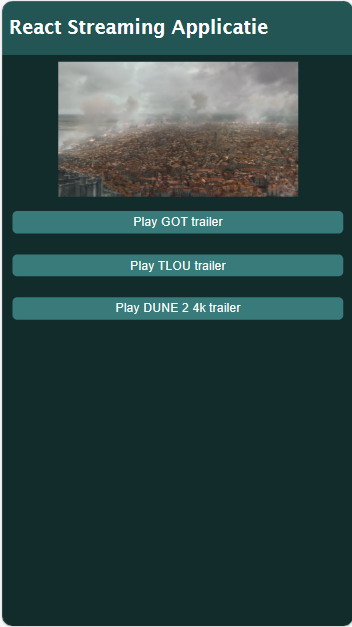
\includegraphics[width=0.7\linewidth]{img/ReactWebsiteIphone}
  \caption{React-website op een iPhone SE vanuit de browser.}
  \label{fig:React-website op een iPhone SE vanuit de browser}
\end{figure}

De volgende en ook wel belangrijkste component in dit POC, is de VideoPlayer-component. Deze is verantwoordelijk voor het effectief afspelen van de geselecteerde video. Deze ontvangt ten eerste een 'videoId' als parameter. Wanneer de 'videoId' zou veranderen in de App-component, zoals bij het aanklikken van een van bovenstaande knoppen, zal deze component volledig opnieuw renderen.

De VideoPlayer maakt daarnaast eerst en vooral gebruik van de 'useRef'-hook om een referentie te verkrijgen naar het <video>-element. Dit is nodig om toegang te verkrijgen tot de video zelf en om bepaalde eigenschappen te kunnen wijzigen. Dit wordt gedaan in de 'useEffect'-hook van de code. Het nut van deze hook is dat deze wordt aangeroepen na de eerste render van de component en na elke volgende update. Dit laat toe om bepaalde side-effects op te lossen. De rol van deze hook heeft vooral te maken met het re-renderen van de VideoPlayer indien de 'videoId' verandert. In dit geval zal de video gepauzeerd worden, de huidige source naar de video verwijderd worden en de video met de nieuwe source correct laden en afspelen. Zonder deze useEffect-hook zou indien een nieuwe video geselecteerd is, deze niet kunnen ingeladen worden en nog steeds een referentie hebben naar de oude source.

Tot slot retourneert deze component een <video>-element waarin de video wordt afgespeeld. De grootte van het video-element wordt dynamisch ingesteld op basis van de 'vidWidth' en 'vidHeight'-states uit de component. De source van de video wordt dynamisch toegekend aan de hand van een url naar de back-end API endpoint met de 'videoId' als parameter.

De code van de VideoPlayer ziet er als volgt uit. Om de leesbaarheid te verhogen tot enkel de belangrijkste aspecten uit de code, zijn enkele lijntjes code weggelaten die betrekking hebben tot de grootte van het venster van de video zelf. Deze hebben echter geen invloed op de prestaties van de website en/of applicatie zelf en behoren ook niet tot de scope van dit onderzoek. Let hierbij op dat de url naar de back-end deels is vervangen door de letter 'X' om privacyredenen. Dit kan vervangen worden door 'localhost', maar bleek de enige oplossing voor de Ionic-applicatie om lokaal de back-end te bereiken.

\begin{mdframed}[backgroundcolor=bg]
  \begin{minted}[breaklines]{jsx}
const VideoPlayer = ({videoId}) => {
    // Referentie naar het video-element
    const videoRef = useRef(null);

    // UseEffect om de video te laden en af te spelen
    // wanneer de videoId verandert (enkel bij de eerste render)
    useEffect(() => {
      if (videoRef.current) {
        videoRef.current.pause();
        videoRef.current.removeAttribute('src');
        videoRef.current.load();
      }
    });

    // Retourneren van de JSX met het video-element
    return (
      <video ref={videoRef} width={vidWidth} height={vidHeight} controls>
        <source src={`http://192.168.X.XXX:3000/videos/\${videoId}`}
          type="video/mkv"></source>
        Your browser does not support the video tag.
      </video>
    );
}
  \end{minted}
\end{mdframed}


\subsection{Ionic applicatie}
\label{sec:ionic-applicatie}

Nu de React-website is opgezet, kan er overgegaan worden tot het ontwikkelen en/of omzetten naar de mobiele applicaties. Uit Hoofdstuk \ref{sec:ionic} bleek dat er eigenlijk geen verdere aanpassingen hoeven te gebeuren aan de bestaande React-website om deze te kunnen omzetten naar een Ionic-applicatie. Ter verduidelijking werd er voor deze Ionic-applicatie gebruik gemaakt van het React-framework, alhoewel er hiervoor ook de keuze is om een andere, door Ionic ondersteund framework, te gebruiken. Dit heeft als troef dat de originele website-codebase letterlijk kan worden hergebruikt voor de mobiele applicatie.

Deze conversie gebeurt aan de hand van de Capacitor-plugin v6.0.0. De Ionic-applicatie zelf is dan weer gebouwd met versie 7.2.0 van Ionic. De combinatie van deze twee plugins maakt het mogelijk om de React-website te converteren naar een native-applicatie voor Android. Dit wordt bereikt door het aanmaken van twee bestanden: \verb|ionic.config.json| en \verb|capacitor.config.json|. Dit eerste bestand bevat the instellingen voor de Ionic-applicatie, zoals de naam en het feit dat deze applicatie steunt op React. Dit ziet er als volgt uit:

\begin{mdframed}[backgroundcolor=bg]
  \begin{minted}[breaklines]{json}
{
  "name": "IonicStreaming",
  "integrations": {
    "capacitor": {}
  },
  "type": "react"
}
  \end{minted}
\end{mdframed}

Het tweede bestand bevat dan weer configuraties voor de Capacitor-plugin. De inhoud hiervan ziet er zo uit:

\begin{mdframed}[backgroundcolor=bg]
  \begin{minted}[breaklines]{json}
{
  "appId": "io.ionic.IonicStreaming",
  "appName": "IonicStreaming",
  "bundledWebRuntime": false,
  "npmClient": "npm",
  "webDir": "build",
  "cordova": {}
}
  \end{minted}
\end{mdframed}

Na het aanmaken van deze bestanden is het nodig om de huidige website eerst te builden. Dit komt omdat Capacitor geen ingebouwde build-tool heeft en gebruik maakt van de bestaande build van de React-website. Door het commando \verb|npm run build| uit te voeren, worden de nodige bestanden gegenereerd in de 'build'-map in de root folder van het project. Er rest nog een laatste stap en dat is het effectief converteren naar een Android-applicatie. Het commando \verb|ionic capacitor| \verb|add android| zorgt hiervoor.

Nadat deze applicatie is geconverteerd, hebben we onze definitieve Ionic-applicatie. Dit zonder enig lijntje van de originele codebase aan te passen. De applicatie kan nu worden gebuild via Gradle en geïnstalleerd op een Android-toestel. Er is echter nog een klein probleem bij deze build en dit heeft allemaal te maken met de lokaal draaiende back-end. Omdat deze via de localhost bereikbaar is, moet het commando \verb|ionic cap run android| \verb|-l --external| worden uitgevoerd. Dit is enkel en alleen nodig in dit specifieke geval: indien de API-endpoint bereikbaar is via een externe HTTPS-verbinding, is dit niet nodig. Wat dit commando doet is de vorige stappen zelf opnieuw uitvoeren, maar de applicatie bovendien ook lokaal draaien op localhost. Dit kan best vergeleken worden met de Ionic-applicatie te draaien op een bepaalde poort, zoals de originele React-website zou doen. Door deze tussenstap te nemen, kan de app opgestart worden met Android Studio en toch de back-end via de lokale pc bereiken.

Een screenshot van de applicatie staat op de volgende pagina.

Door deze bovenstaande stappen te volgen was het dus mogelijk om zonder enige aanpassingen, de React-website te deployen als een native Android-applicatie. Dit toont aan dat de combinatie van React, Ionic en Capacitor een krachtige toolset is om webapplicaties om te zetten naar mobiele applicaties. Wat natuurlijk weer een voordeel is voor ontwikkelaars om niet een volledig nieuwe applicatie te moeten herimplementeren.

\subsection{React Native applicatie}
\label{sec:react-native-applicatie}

Het laatste deel van de opzetting voor de testscenario's is de React Native-conversie. In tegenstelling tot een Ionic-applicatie, steunt deze niet op de typische webtechnologie van HTML, maar maakt gebruikt van eigen custom componenten. Dit wil betekenen dat de React-website niet zomaar kan worden omgezet naar een React Native-applicatie zoals bij Ionic. Desondanks is deze omzetting wel mogelijk omdat React Native voor de meeste HTML-elementen een equivalent heeft. Dit laat toe om de meeste code toch op een relatief eenvoudige manier te kunnen hergebruiken, mits enkele aanpassingen die hier worden besproken.

\begin{figure}
  \centering
  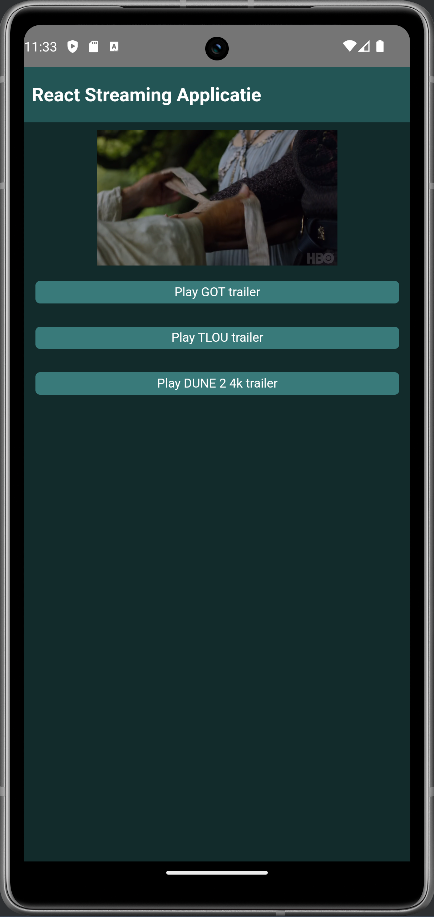
\includegraphics[width=0.7\linewidth]{img/ReactIonicPhone}
  \caption{Ionic-applicatie op een Google Pixel 7a}
  \label{fig:Ionic-applicatie op een Google Pixel 7a}
\end{figure}

\begin{mdframed}[backgroundcolor=bg]
  \begin{minted}[breaklines]{jsx}
const App = () => {
    // State voor de videoId
    const [videoId, setVideoId] = useState(null);

    // Functie om een video af te spelen bij het klikken
    // op een knop
    function playVideo(e, videoId) {
      e.preventDefault();
      setVideoId(videoId);
    };

    // Retourneren van de JSX met de Header-, VideoPlayer-
    // en Button-componenten
    return (
      <View style={styles.app}>
        <Header />
        <View style={styles.content}>
            <VideoPlayer videoId={videoId}></VideoPlayer>
            <View style={styles.vidSelect}>
              <Button
                onPress={(e) => playVideo(e, 'got')}
                title='Play GOT trailer'
                color={'rgb(57, 122, 122)'}>
              </Button>
              <Button
                onPress={(e) => playVideo(e, 'tlou')}
                title='Play TLOU trailer'
                color={'rgb(57, 122, 122)'}>
              </Button>
              <Button
                onPress={(e) => playVideo(e, 'dune')}
                title='Play DUNE 2 4k trailer'
                color={'rgb(57, 122, 122)'}>
              </Button>
          </View>
        </View>
      </View>
    );
};
  \end{minted}
\end{mdframed}

Bovenstaande code toont de App-component van de React Native-applicatie. Deze is zeer gelijkaardig aan de App-component van de originele React-website. Het grootste verschil is dat de HTML-elementen vervangen zijn door React Native- componenten. Zo wordt de <div>-tag vervangen door de <View>-tag en de HTML-buttons door de <Button>-component. De styling werd ook identiek overgezet op basis van de React-website, maar heeft eigenlijk geen invloed op de werking van de applicatie zelf. Als er vervolgens gekeken wordt naar de VideoPlayer-component, is deze ook gelijkaardig opgebouwd als de React-website. Maar voor deze component bleek er toch één groot probleem: React Native biedt geen standaard video-component aan. Dit betekent dus dat er moet gesteund worden op een externe package. In dit geval werd er gekozen voor de 'react-native-video'-package. Deze light-weight package biedt een video-component aan die zeer gelijkaardig is aan de <video>-tag in HTML.

Er wordt daarnaast opnieuw gebruikt gemaakt van de 'useRef'-hook om een referentie te verkrijgen naar het video-element. De useEffect-hook bij Ionic wordt echter niet gebruikt aangezien de React Native-video-component zelf al een ingebouwde manier heeft om de video te pauzeren en te hervatten, en de source van de video automatisch laat wijzigen wanneer de 'videoId' verandert. Deze useEffect-hook is dus overbodig in dit geval.

Voor de connectie met localhost is er geen extra configuratie nodig zoals bij de Ionic-applicatie. Slechts de url zoals in de onderstaande code bleek voldoende voor de connectie:

\begin{figure}
  \centering
  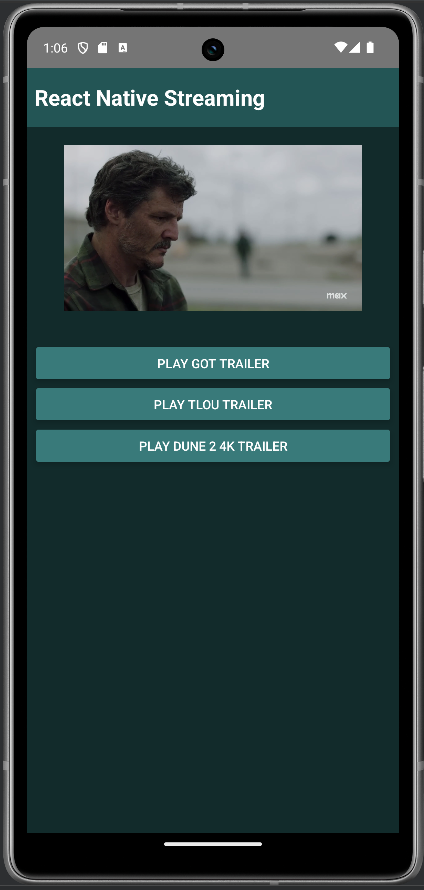
\includegraphics[width=0.7\linewidth]{img/ReactNativePhone}
  \caption{React Native-applicatie op een Google Pixel 7a}
  \label{fig:React Native-applicatie op een Google Pixel 7a}
\end{figure}

\begin{mdframed}[backgroundcolor=bg]
  \begin{minted}[breaklines]{jsx}
const VideoPlayer = ({videoId}) => {
    // Referentie naar het video-element
    const videoRef = useRef(null);

    // Retourneren van de JSX met de video-component
    // van de react-native-video package
    return (
      <View style={styles.videoView}>
        <Video 
          source={{uri: `http://10.0.2.2:3000/videos/${videoId}`}} 
          ref={(ref) => {
            videoRef.current = ref;
          }}         
          style={styles.backgroundVideo}
        />
      </View>
    );
}
  \end{minted}
\end{mdframed}

Nu de code is geschreven is het enkel nog een kwestie van de applicatie te builden en te deployen naar een Android-toestel. Hiervoor werd er in de package.json volgende script toegevoegd:

\begin{mdframed}[backgroundcolor=bg]
  \begin{minted}[breaklines]{json}
"build": "react-native bundle --platform android --dev false --entry-file index.js --bundle-output android/app/src/main/assets/index android.bundle --assets-dest android/app/src/main/res"
  \end{minted}
\end{mdframed}

%++ metro v0.80.8

Dit script zorgt ervoor dat de code wordt gebundeld en dat de nodige bestanden worden gegenereerd in de 'android/app/src/main/assets'-map van de root-folder. Vervolgens kan deze build worden geopend in Android Studio en kan de applicatie via Gradle worden gebuild en geïnstalleerd op een Android-toestel. De afbeelding op de vorige pagina toont de React Native-applicatie op een Google Pixel 7a. Enkele verschillen zijn misschien merkbaar in de styling tussen de verschillende versies, maar dit heeft opnieuw geen invloed op de performantie van de applicatie en eerder te maken met de beperkte styling die React Native aan zijn componenten geeft. Bovendien werd de styling zo goed als helemaal overgenomen van de originele React-website (en dus ook Ionic-applicatie), dus deze kleine verschillen zijn als het ware verwaarloosbaar.

\section{Testscenario's}
\label{sec:testscenario}

Gezien de ontwikkeling van zowel de Ionic- als de React Native-applicaties nu voltooid is, kan er overgegaan worden naar de testfase van deze Proof-of-Concept. In deze fase zal er onder andere gekeken worden naar de algemene opstarttijden, gebruikerservaring bij de interactie met de applicatie, alsook metingen worden gedaan met betrekking tot het CPU- en geheugenverbruik.


\subsection{Cold startup-tijd}
\label{subsec:cold-startup-tijd}

De term cold startup-tijd verwijst naar de tijd die nodig is voor een applicatie om op te starten vanaf het begin. Dit in een situatie waarbij de applicatie nog niet is geopend (zoals bij het opstarten van het toestel) of na het volledig afsluiten van de app. Deze meting werd uitgevoerd door de applicatie eerst telkens volledig af te sluiten door een 'force stop' uit te voeren op de emulator en vervolgens de applicatie opnieuw te openen. Aan de hand van de logs en de Profiler van Android Studio kon de tijd gemeten worden vanaf het aanklikken van het icoon, tot wanneer de componenten volledig zijn ingeladen op het scherm. Er valt hierbij op te merken dat de videocomponent nog niet wordt ingeladen vanwege het feit dat er geen video is geselecteerd. Dit wordt in een latere fase onderzocht.

Dit waren de resultaten na twintig metingen:

\begin{table}[htbp]
  \centering
  \begin{tabular}{|c|c|c|}
    \hline
    \textbf{Testscenario} & \textbf{Ionic} & \textbf{React Native} \\
    \hline
    1 & 2s 961ms & 6s 539ms \\
    \hline
    2 & 3s 114ms & 6s 876ms \\
    \hline
    3 & 3s 191ms & 6s 967ms \\
    \hline
    4 & 2s 987ms & 6s 477ms \\
    \hline
    5 & 3s 73ms & 6s 826ms \\
    \hline
    6 & 3s 118ms & 6s 895ms \\
    \hline
    7 & 2s 953ms & 6s 488ms \\
    \hline
    8 & 3s 2ms & 6s 611ms \\
    \hline
    9 & 3s 112ms & 6s 524ms \\
    \hline
    10 & 3s 148ms & 6s 450ms \\
    \hline
    11 & 3s 13ms & 6s 868ms \\
    \hline
    12 & 3s 205ms & 6s 813ms \\
    \hline
    13 & 2s 914ms & 6s 742ms \\
    \hline
    14 & 2s 902ms & 6s 499ms \\
    \hline
    15 & 3s 55ms & 6s 981ms \\
    \hline
    16 & 3s 70ms & 6s 827ms \\
    \hline
    17 & 2s 845ms & 6s 879ms \\
    \hline
    18 & 3s 113ms & 6s 624ms \\
    \hline
    19 & 2s 947ms & 6s 760ms \\
    \hline
    20 & 3s 6ms & 6s 855ms \\
    \hline
    \textbf{Gemiddelde} & \textbf{3s 36ms} & \textbf{6s 725ms} \\
    \hline
  \end{tabular}
  \caption{Cold startup tijd voor Ionic en React Native applicaties}
  \label{tab:cold_startup}
\end{table}

\begin{figure}
  \centering
  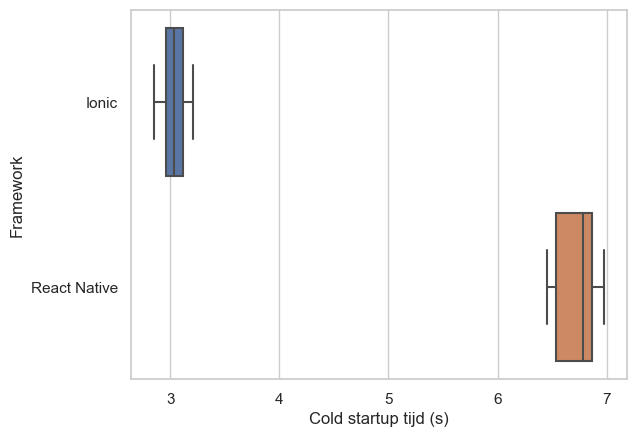
\includegraphics[width=0.7\linewidth]{img/boxplotCold}
  \caption{Boxplot van de cold startup-tijd voor Ionic en React Native applicaties}
  \label{fig:Boxplot van de cold startup-tijd voor Ionic en React Native applicaties}
\end{figure}

Deze resultaten werden vervolgens in een boxplot weergegeven om een beter beeld te verkrijgen van de spreiding van de data. Dit wordt weergegeven in het bovenstaande Figuur \ref{fig:Boxplot van de cold startup-tijd voor Ionic en React Native applicaties}. Vervolgens werd er een t-test uitgevoerd om aan te tonen of er een significant verschil is tussen de gemiddelden van de cold startup-tijden bij Ionic en React Native. Als nulhypothese werd er vastgelegd dat er geen significant verschil is tussen de gemiddelden. De alternatieve hypothese, op basis van de boxplot en de tabel, was dat de resultaten voor Ionic lager zouden zijn dan die van React Native. De analyse werd uitgevoerd met een vastgesteld significantieniveau van \(0.05\). Uit deze test bleek dat de p-waarde \(1.312^{-36}\) bedroeg. Dit is aanzienlijk lager dat het significantieniveau en betekent dat de nulhypothese kan worden verworpen. Dit wijst er bovendien op dat de cold startup-tijden afhankelijk zijn van het type framework en dat Ionic inderdaad over significant snellere cold startup-tijden beschikt dan React Native. Dit kan een belangrijke factor zijn voor de gebruikerservaring van een applicatie. Een verdere verklaring en interpretatie van deze resultaten wordt, zoals eerder vermeld, gegeven in het volgende hoofdstuk.


\subsection{Warm startup-tijd}
\label{subsec:warm-startup-tijd}

Warm startup-tijd verwijst naar de tijd die nodig is voor een applicatie om opnieuw te starten nadat deze al een keer is gestart geweest en enige tijd inactief is. Dit is te vergelijken met een gebruiker die de applicatie opnieuw opent nadat deze al een keer is geopend en vervolgens is geminimaliseerd, om bijvoorbeeld te surfen op het internet. Dit omvat dus het opnieuw inladen van de applicatie, waarbij de resources voor een deel of volledig nog in het geheugen zijn opgeslagen. Deze meting werd uitgevoerd door de applicatie te openen, te minimaliseren, Google Chrome te openen en weer te minimaliseren, en vervolgens de Ionic- of React Native-app weer te openen. De tijd werd gemeten vanaf het aanklikken van het icoon tot wanneer de componenten volledig zijn ingeladen op het scherm op basis van de logs en de Profiler van Android Studio.

\begin{table}[htbp]
  \centering
  \begin{tabular}{|c|c|c|}
  \hline
  \textbf{Testscenario} & \textbf{Ionic} & \textbf{React Native} \\
  \hline
  1 & 239ms & 239ms \\
  \hline
  2 & 328ms & 237ms \\
  \hline
  3 & 301ms & 195ms \\
  \hline
  4 & 283ms & 232ms \\
  \hline
  5 & 241ms & 217ms \\
  \hline
  6 & 319ms & 200ms \\
  \hline
  7 & 281ms & 231ms \\
  \hline
  8 & 252ms & 204ms \\
  \hline
  9 & 302ms & 218ms \\
  \hline
  10 & 275ms & 245ms \\
  \hline
  11 & 236ms & 209ms \\
  \hline
  12 & 241ms & 233ms \\
  \hline
  13 & 291ms & 241ms \\
  \hline
  14 & 212ms & 226ms \\
  \hline
  15 & 333ms & 191ms \\
  \hline
  16 & 276ms & 221ms \\
  \hline
  17 & 273ms & 231ms \\
  \hline
  18 & 299ms & 208ms \\
  \hline
  19 & 269ms & 221ms \\
  \hline
  20 & 305ms & 213ms \\
  \hline
  \textbf{Gemiddelde} & \textbf{278ms} & \textbf{221ms} \\
  \hline
  \end{tabular}
  \caption{Warm startup-tijd voor Ionic en React Native applicaties}
  \label{tab:warm_startup}
\end{table}

\begin{figure}
  \centering
  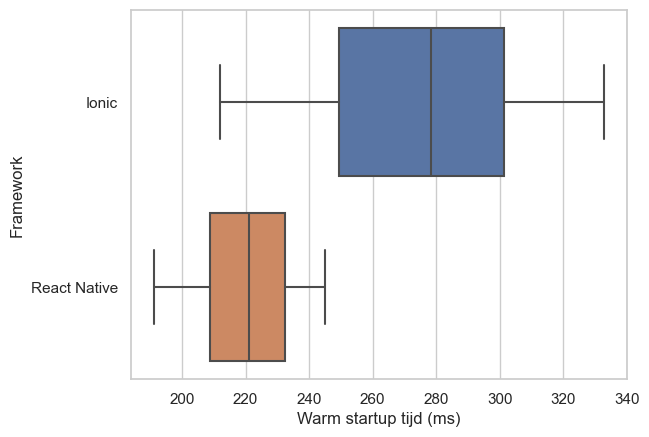
\includegraphics[width=0.7\linewidth]{img/boxplotWarm}
  \caption{Boxplot van de warm startup-tijd voor Ionic en React Native applicaties}
  \label{fig:Boxplot van de warm startup-tijd voor Ionic en React Native applicaties}
\end{figure}

Ook voor deze gegevens werd er een boxplot gemaakt (zie Figuur \ref{fig:Boxplot van de warm startup-tijd voor Ionic en React Native applicaties}). Vervolgens werd er opnieuw een t-test uitgevoerd om te zien of er een significant verschil is tussen de gemiddelden van de warm startup-tijden bij beide frameworks. De nulhypothese was dat er geen verschil is tussen de gemiddelden en als alternatieve hypothese dat de resultaten voor React Native lager zouden zijn dan die van Ionic. Deze test werd opnieuw uitgevoerd met een significantieniveau van \(0.05\). De p-waarde had als waarde \(8.244^{-8}\), wat lager is dan de significantieniveau. Hieruit kan geconcludeerd worden dat de nulhypothese kan verworpen worden en dat React Native over het algemeen iets sneller blijkt te zijn dan Ionic, alhoewel dit verschil slechts over enkele milliseconden gaat en eigenlijk op gebruikersniveau quasi 


\subsection{Interactie}
\label{subsec:interactie}

De interactie met de applicaties werd als vrij responsief ervaren. Het was mogelijk om vrij snel te schakelen tussen de verschillende video's door op de knoppen te klikken. Vanaf een knop werd aangeklikt, reageerde de interface onmiddellijk door de videospeler te renderen en binnen een tijdspanne van 2-3 seconden de video af te spelen. Ondanks dat er een pauze was tussen het klikken op de knop en het effectief inladen van de video, werd deze pauze niet als storend ervaren en werd de video snel en vloeiend afgespeeld. Bij het meten werd er deze keer opnieuw gekeken naar de Android Profiler en de logs van Android Studio om de reactietijden te meten. De resultaten van deze metingen zijn te vinden in de volgende tabel.

%erbij vermelden dat emulator stottert


\begin{table}[htbp]
  \centering
  \begin{tabular}{|c|c|c|}
  \hline
  \textbf{Testscenario} & \textbf{Ionic} & \textbf{React Native} \\
  \hline
  1 & 2s 807ms & 3s 56ms \\
  \hline
  2 & 2s 159ms & 2s 218ms \\
  \hline
  3 & 2s 123ms & 3s 177ms \\
  \hline
  4 & 2s 412ms & 2s 979ms \\
  \hline
  5 & 2s 788ms & 2s 762ms \\
  \hline
  6 & 2s 437ms & 2s 731ms \\
  \hline
  7 & 2s 354ms & 2s 964ms \\
  \hline
  8 & 2s 617ms & 2s 916ms \\
  \hline
  9 & 2s 622ms & 2s 775ms \\
  \hline
  10 & 2s 201ms & 2s 549ms \\
  \hline
  11 & 2s 193ms & 2s 636ms \\
  \hline
  12 & 2s 773ms & 2s 985ms \\
  \hline
  13 & 2s 111ms & 2s 909ms \\
  \hline
  14 & 2s 479ms & 3s 41ms \\
  \hline
  15 & 2s 671ms & 2s 963ms \\
  \hline
  16 & 2s 306ms & 2s 843ms \\
  \hline
  17 & 2s 828ms & 2s 872ms \\
  \hline
  18 & 2s 584ms & 2s 469ms \\
  \hline
  19 & 2s 453ms & 2s 760ms \\
  \hline
  20 & 2s 404ms & 2s 932ms \\
  \hline
  \textbf{Gemiddelde} & \textbf{2s 466ms} & \textbf{2s 827ms} \\
  \hline
  \end{tabular}
  \caption{Tijd voor het inladen van de video na het klikken op een knop voor Ionic en React Native applicaties}
  \label{tab:warm_startup}
\end{table}

\begin{figure}
  \centering
  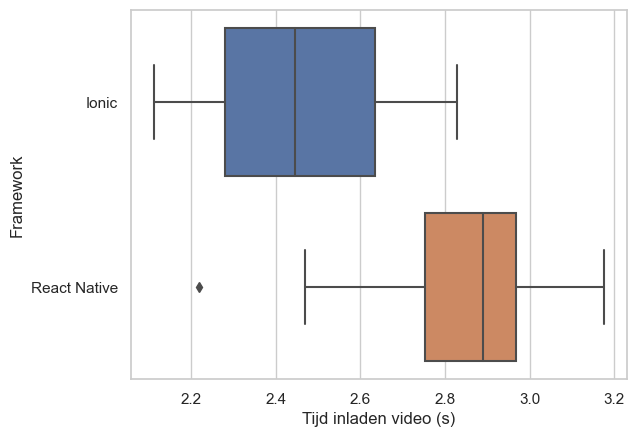
\includegraphics[width=0.7\linewidth]{img/boxplotInteraction}
  \caption{Boxplot van de tijd voor het inladen van de video na het klikken op een knop voor Ionic en React Native applicaties}
  \label{fig:Boxplot van de tijd voor het inladen van de video na het klikken op een knop voor Ionic en React Native applicaties}
\end{figure}

Indien voor dit testscenario opnieuw de t-test uitgevoerd wordt met een significantieniveau van \(0.05\), krijgt de p-waarde een waarde van \(8.624^{-6}\). Dit is opnieuw lager dan het significantieniveau en betekent dat ook hier Ionic een kleine voorsprong heeft op React Native. Op zich lijkt dit verschil misschien op het eerste zicht niet zo groot, maar in een situatie waarbij de gebruiker snel wilt schakelen tussen verschillende video's, om bijvoorbeeld de juiste video te vinden, kan dit na enkele keren toch wel een merkbaar verschil beginnen worden tussen beide applicaties. Vanwege deze reden wordt Ionic hier als een betere keuze beschouwd op vlak van het ophalen en inladen van de video's.


\subsection{Video afspeelprestaties}
\label{subsec:video-afspeelprestaties}

Bij het afspelen van video's op zowel React als Ionic, werd over het algemeen een hoge afspeelkwaliteit ervaren. De video's werd telkens in hoge kwaliteit met een goed geluid afgespeeld. Echter werden er momenten waargenomen waarbij er enige haperingen optraden, vooral bij het afspelen van video's met de hogere resolutie van 4k. Hierdoor begon ook de geluidssynchronisatie het wat te begeven en leek het aanvankelijk alsof beide applicaties wel wat moeite bleken te hebben.

Echter op basis van onderstaande metingen, blijkt dat de haperingen eerder te wijten zijn aan de emulator dan aan de applicaties zelf. Dit wordt ondersteund door observaties van het CPU-gebruik die op geen enkel moment werd overbelast. Daarnaast hapert de emulator zelf ook bij het algemeen gebruik, zoals bij het scrollen tussen de geïnstalleerde applicaties, met andere woorden bij laag intensief gebruik.


\subsection{CPU-gebruik}
\label{subsec:cpu-gebruik}

Het CPU-gebruik werd telkens als volgt gemeten. Allereerst werd de applicatie de eerste keer opgestart nadat deze volledig was afgesloten. Vervolgens werd de eerste meting uitgevoerd totdat de applicatie volledig was opgestart. Aan de hand van de Android Profiler in Android Studio werd er gekeken naar het CPU-gebruik van de applicatie en werd hiervan het gemiddelde genomen. De volgende test werd uitgevoerd nadat de app was opgestart, met andere woorden wanneer de app "idle" was en gebeurde telkens over een periode van exact 5 seconden. Hierna werden beide 1080p video's getest en als laatste de 4k video, telkens begon de meting vanaf het aanklikken van de knop tot exact 5 seconden later, wanneer de video al enkele seconden aan het afspelen was. Ook hiervan werd er telkens het gemiddelde genomen van het CPU-gebruik. Deze metingen werden een vijftiental keer herhaald om een beter beeld te verkrijgen van de variabiliteit van de data.

%Het CPU-gebruik werd telkens als volgt gemeten. Allereerst werd de applicatie de eerste keer opgestart nadat deze volledig was afgesloten. Vervolgens werd er een meting gedaan zonder dat er een video werd afgespeeld. Hierna werden beide 1080p video's getest en als laatste de 4k video. De metingen werden gedaan aan de hand van de Android Profiler in Android Studio. Hierbij werd er gekeken naar de CPU-gebruikspieken en -dalen die optraden tijdens de verschillende activiteiten.

%Voor Ionic vertoonde de applicatie bij het opstarten een piek van 41\% CPU-gebruik. Zonder het afspelen van video's bleef het CPU-gebruik hierna tussen 0-1\%. Bij het afspelen van een 1080p video varieerde het CPU-gebruik tussen 22-37\%, met enkele dalingen van 12\% en pieken tot 43\% van het totale CPU-gebruik. Bij het afspelen van een 4k video waren er iets hogere variaties tussen 32-52\%, met een drop van 32\% en een piek van 68\%.

%Bij de observatie van het CPU-gebruik bij React Native tijdens dezelfde activiteiten, valt op dat er bij het starten van de applicatie een piek van 50\% CPU-gebruik optreedt. Dit is een gelijkaardige piek zoals bij Ionic. Zonder het afspelen van video's bleef het CPU-gebruik tussen de 1-2\% zitten. Wanneer een 1080p video werd afgespeeld, varieert het CPU-gebruik tussen 35-41\% bij het inladen van de video en varieerde vervolgens tussen de 38-70\%, met enkele dalingen tot 20\% en hoge pieken tot zelfs 90\%. Bij het afspelen van een 4k video varieerde dit ook vrij hard, met een dieptepunt van 26\% en een piek van 92\%, en een algemene variatie tussen 35-82\%. 

%Over het algemeen tonen deze observaties aan dat het CPU-gebruik vrij hoog kan zijn bij het afspelen van video's, vooral bij hogere resoluties zoals 4k. Dit kan leiden tot een hoger energieverbruik en een snellere batterijafvoer, wat belangrijk is om in overweging te nemen bij het ontwikkelen van video-intensieve applicaties. Daarnaast bleek ook dat React Native telkens een hoger CPU-gebruik had dan Ionic. Een mogelijke verklaring wordt later besproken.


\begin{table}[htbp]
  \centering
  \footnotesize
  \begin{tabular}{|c|c|c|c|c|}
      \hline
      \textbf{Testscenario} & \textbf{Startup I (\%)} & \textbf{Startup RN (\%)} & \textbf{Opgestart I (\%)} & \textbf{Opgestart RN (\%)} \\
      \hline
      1 & 30 & 21 & 0 & 1 \\
      \hline
      2 & 33 & 20 & 1 & 1 \\
      \hline
      3 & 29 & 22 & 1 & 0 \\
      \hline
      4 & 32 & 20 & 0 & 1 \\
      \hline
      5 & 30 & 18 & 0 & 0 \\
      \hline
      6 & 32 & 20 & 0 & 0 \\
      \hline
      7 & 28 & 19 & 1 & 1 \\
      \hline
      8 & 34 & 20 & 0 & 0 \\
      \hline
      9 & 26 & 21 & 1 & 1 \\
      \hline
      10 & 30 & 20 & 0 & 1 \\
      \hline
      11 & 28 & 21 & 0 & 1 \\
      \hline
      12 & 33 & 19 & 1 & 1 \\
      \hline
      13 & 30 & 20 & 1 & 0 \\
      \hline
      14 & 32 & 20 & 0 & 1 \\
      \hline
      15 & 28 & 19 & 1 & 0 \\
      \hline
      \textbf{Gemiddelde} & \textbf{30.3} & \textbf{20} & \textbf{0.47} & \textbf{0.60} \\
      \hline
  \end{tabular}
  \caption{CPU-gebruik van de Ionic en React Native applicaties bij het opstarten (Startup) en wanneer de applicatie opgestart is (Opgestart). Hierbij verwijst de letter 'I' naar Ionic en 'RN' naar React Native.}
  \label{tab:cpu1}
\end{table}

\begin{table}[htbp]
  \centering
  \footnotesize
  \begin{tabular}{|c|c|c|c|c|c|c|}
      \hline
      \textbf{Testscenario} & \textbf{HD-1 I (\%)} & \textbf{HD-1 RN (\%)} & \textbf{HD-2 I (\%)} & \textbf{HD-2 RN (\%)} & \textbf{UHD I (\%)} & \textbf{UHD RN (\%)} \\
      \hline
      1 & 20 & 32 & 22 & 40 & 51 & 56 \\
      \hline
      2 & 18 & 31 & 24 & 44 & 38 & 63 \\
      \hline
      3 & 26 & 35 & 19 & 34 & 42 & 61 \\
      \hline
      4 & 21 & 29 & 23 & 29 & 59 & 70 \\
      \hline
      5 & 21 & 33 & 25 & 36 & 39 & 65 \\
      \hline
      6 & 19 & 30 & 25 & 28 & 56 & 60 \\
      \hline
      7 & 23 & 36 & 22 & 31 & 34 & 50 \\
      \hline
      8 & 16 & 34 & 26 & 38 & 48 & 71 \\
      \hline
      9 & 24 & 28 & 23 & 45 & 46 & 62 \\
      \hline
      10 & 19 & 29 & 20 & 33 & 52 & 69 \\
      \hline
      11 & 20 & 30 & 24 & 40 & 57 & 75 \\
      \hline
      12 & 16 & 31 & 21 & 38 & 38 & 73 \\
      \hline
      13 & 22 & 33 & 25 & 27 & 55 & 57 \\
      \hline
      14 & 18 & 32 & 24 & 34 & 43 & 66 \\
      \hline
      15 & 23 & 30 & 19 & 41 & 50 & 52 \\
      \hline
      \textbf{Gemiddelde} & \textbf{20.4} & \textbf{31.5} & \textbf{22.8} & \textbf{35.9} & \textbf{47.2} & \textbf{63.3} \\
      \hline
  \end{tabular}
  \caption{CPU-gebruik van de Ionic en React Native applicaties bij het afspelen van video's. De letter 'I' verwijst naar Ionic en 'RN' naar React Native respectievelijk.}
  \label{tab:cpu2}
\end{table}

\begin{figure}
  \centering
  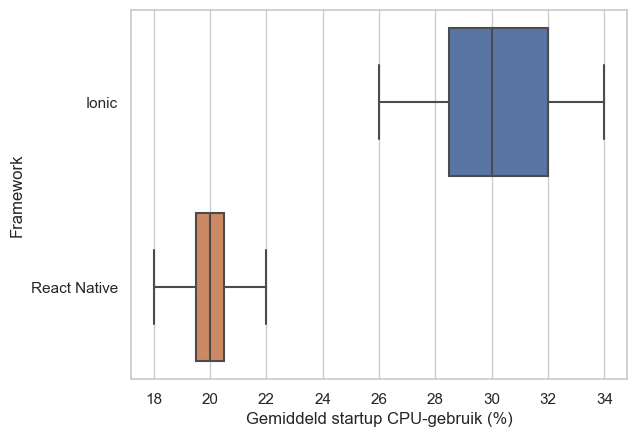
\includegraphics[width=0.7\linewidth]{img/cpu/startup}
  \caption{Boxplot van het CPU-gebruik van de Ionic en React Native applicaties bij het opstarten}
  \label{fig:Boxplot van het CPU-gebruik van de Ionic en React Native applicaties bij het opstarten}
\end{figure}

\begin{figure}
  \centering
  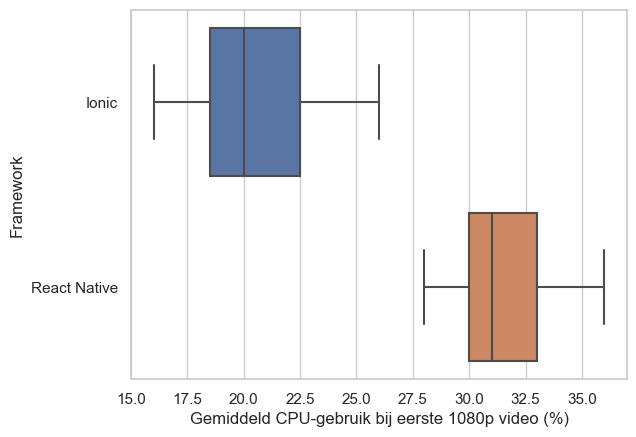
\includegraphics[width=0.7\linewidth]{img/cpu/HD1}
  \caption{Boxplot van het CPU-gebruik van de Ionic en React Native applicaties bij het afspelen van de eerste 1080p video}
  \label{fig:Boxplot van het CPU-gebruik van de Ionic en React Native applicaties bij het afspelen van de eerste 1080p video}
\end{figure}

\begin{figure}
  \centering
  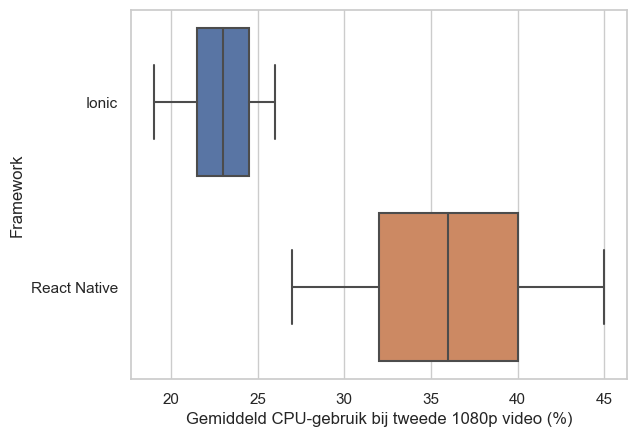
\includegraphics[width=0.7\linewidth]{img/cpu/HD2}
  \caption{Boxplot van het CPU-gebruik van de Ionic en React Native applicaties bij het afspelen van de tweede 1080p video}
  \label{fig:Boxplot van het CPU-gebruik van de Ionic en React Native applicaties bij het afspelen van de tweede 1080p video}
\end{figure}

\begin{figure}
  \centering
  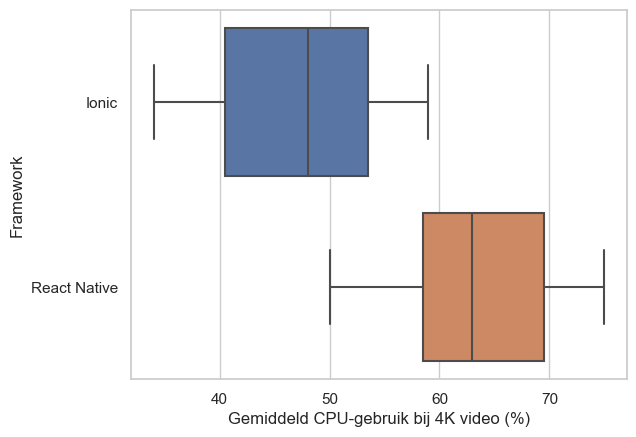
\includegraphics[width=0.7\linewidth]{img/cpu/4k}
  \caption{Boxplot van het CPU-gebruik van de Ionic en React Native applicaties bij het afspelen van de 4k video}
  \label{fig:Boxplot van het CPU-gebruik van de Ionic en React Native applicaties bij het afspelen van de 4k video}
\end{figure}


Bij het opstarten van de applicatie vertoonde de Ionic-applicatie een vrij hoger gemiddeld CPU-gebruik in tegenstelling tot React Native. Dit is te zien in de bovenstaande tabel \ref{tab:cpu1} en de bijhorende boxplot in Figuur \ref{fig:Boxplot van het CPU-gebruik van de Ionic en React Native applicaties bij het opstarten}. Echter eens beide applicaties waren opgestart, bleef het CPU-gebruik van beide applicaties ongeveer op hetzelfde niveau hangen, namelijk rond de 0 en 1 procent. Aangezien het hier slechts over een zeer laag percentage gaat en eigenlijk bijna verwaarloosbaar is, werd hier niet dieper op ingegaan. Het is namelijk +++

\begin{table}[htbp]
  \centering
  \footnotesize
  \begin{tabular}{|c|c|c|}
      \hline
      \textbf{Testvideo} & \textbf{P-waarde} & \textbf{Beste resultaat} \\
      \hline
      Eerste HD-video & \(2.574^{-12}\) & Ionic \\
      \hline
      Tweede HD-video & \(5.975^{-8}\) & Ionic \\
      \hline
      UHD-video & \(1.958^{-6}\) & Ionic \\
      \hline
  \end{tabular}
  \caption{Resultaten van de t-test voor het CPU-gebruik bij het afspelen van video's}
  \label{tab:cpu_ttest}
\end{table}

TODO: TABELLEN AFKORTINGEN UITLEGGEN

Voor de resultaten bij het afspelen van de video's waren er toch wat verschillen te merken. Op basis van de grafieken en tabellen bleek Ionic hier steeds de overduidelijke winnaar te zijn. Maar om dit toch statistisch te onderbouwen, werd er een t-test uitgevoerd met als significantieniveau opnieuw \(0.05\). De resultaten hiervan zijn te vinden in de bovenstaande tabel \ref{tab:cpu_ttest}. Hieruit blijkt dat er een significant verschil is tussen het CPU-gebruik van Ionic en React Native bij het afspelen van video's. Uit de tabel \ref{tab:cpu2} kan er bovendien zelf een verband worden gelegd tussen de resolutie van de video en het CPU-gebruik. Zo is het CPU-gebruik bij het afspelen van een 4k video aanzienlijk hoger dan bij een 1080p video.+++


\subsection{Geheugengebruik}
\label{subsec:geheugengebruik}

Het geheugengebruik werd gemeten aan de hand van de Android Profiler in Android Studio. Hierbij werd er gekeken naar het piek-geheugengebruik na het opstarten van de applicatie en bij het afspelen van de video's. De metingen werden telkens gedaan in megabytes (MB) en werden een vijftiental keer herhaald om een beter beeld te krijgen van de variabiliteit van de data.+ reden waarom

\begin{table}[htbp]
  \centering
  \begin{tabular}{|c|c|c|}
      \hline
      \textbf{Testscenario} & \textbf{Opgestart I (MB)} & \textbf{Opgestart RN (MB)} \\
      \hline
      1 & 113.2 & 113.5 \\
      \hline
      2 & 114.6 & 117.2 \\
      \hline
      3 & 115.5 & 115.1 \\
      \hline
      4 & 113.8 & 118.0 \\
      \hline
      5 & 112.4 & 114.3 \\
      \hline
      6 & 112.7 & 119.1 \\
      \hline
      7 & 114.9 & 113.8 \\
      \hline
      8 & 112.8 & 117.5 \\
      \hline
      9 & 115.9 & 116.7 \\
      \hline
      10 & 113.6 & 114.9 \\
      \hline
      11 & 114.1 & 115.3 \\
      \hline
      12 & 113.1 & 117.8 \\
      \hline
      13 & 115.2 & 113.4 \\
      \hline
      14 & 114.3 & 116.1 \\
      \hline
      15 & 112.5 & 118.6 \\
      \hline
      \textbf{Gemiddelde} & \textbf{113.9} & \textbf{116.1} \\
      \hline
  \end{tabular}
  \caption{Piek-geheugengebruik van Ionic en React Native applicaties wanneer de applicatie opgestart is. Hierbij verwijst de letter 'I' naar Ionic en 'RN' naar React Native.}
  \label{tab:memory1}
\end{table}

\begin{table}[htbp]
  \centering
  \footnotesize
  \scalebox{0.9}{
    \begin{tabular}{|c|c|c|c|c|c|c|}
        \hline
        \textbf{Testscenario} & \textbf{HD-1 I (MB)} & \textbf{HD-1 RN (MB)} & \textbf{HD-2 I (MB)} & \textbf{HD-2 RN (MB)} & \textbf{UHD I (MB)} & \textbf{UHD RN (MB)} \\
        \hline
        1 & 121.7 & 136.7 & 120.5 & 133.2 & 122.5 & 149.5 \\
        \hline
        2 & 118.9 & 141.0 & 119.3 & 140.3 & 122.9 & 153.0 \\
        \hline
        3 & 120.2 & 139.8 & 118.7 & 145.7 & 119.9 & 152.4 \\
        \hline
        4 & 121.5 & 137.5 & 118.5 & 142.9 & 121.2 & 151.1 \\
        \hline
        5 & 117.5 & 135.9 & 120.7 & 132.1 & 121.6 & 150.6 \\
        \hline
        6 & 118.3 & 143.2 & 118.4 & 138.5 & 118.8 & 155.2 \\
        \hline
        7 & 121.8 & 148.6 & 117.9 & 145.2 & 121.8 & 154.1 \\
        \hline
        8 & 121.4 & 151.3 & 118.3 & 149.5 & 121.3 & 156.0 \\
        \hline
        9 & 120.1 & 142.1 & 121.5 & 138.7 & 118.6 & 152.7 \\
        \hline
        10 & 119.7 & 137.4 & 118.4 & 136.2 & 121.5 & 150.8 \\
        \hline
        11 & 117.2 & 140.6 & 120.9 & 144.9 & 121.0 & 153.6 \\
        \hline
        12 & 122.2 & 147.2 & 121.2 & 148.3 & 120.9 & 155.7 \\
        \hline
        13 & 118.2 & 135.8 & 120.3 & 133.7 & 121.4 & 149.9 \\
        \hline
        14 & 121.9 & 149.0 & 120.1 & 146.6 & 119.8 & 154.5 \\
        \hline
        15 & 117.4 & 150.1 & 121.0 & 147.5 & 120.3 & 151.3 \\
        \hline
        \textbf{Gemiddelde} & \textbf{119.9} & \textbf{142.4} & \textbf{119.7} & \textbf{141.6} & \textbf{120.9} & \textbf{152.7} \\
        \hline
    \end{tabular}
  }
  \caption{Geheugengebruik voor Ionic en React Native applicaties bij het afspelen van video's. De letter 'I' verwijst naar Ionic en 'RN' naar React Native respectievelijk.}
  \label{tab:memory2}
\end{table}

\begin{figure}
  \centering
  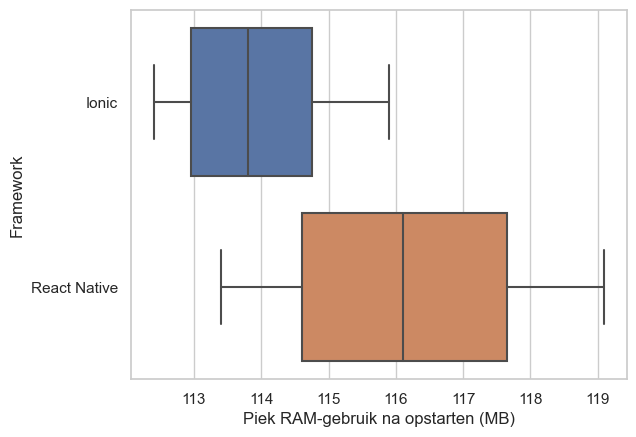
\includegraphics[width=0.7\linewidth]{img/ram/loaded}
  \caption{Boxplot van het piek-geheugengebruik van Ionic en React Native applicaties wanneer de applicatie opgestart is}	
  \label{fig:Boxplot van het piek-geheugengebruik van Ionic en React Native applicaties wanneer de applicatie opgestart is}
\end{figure}

\begin{figure}
  \centering
  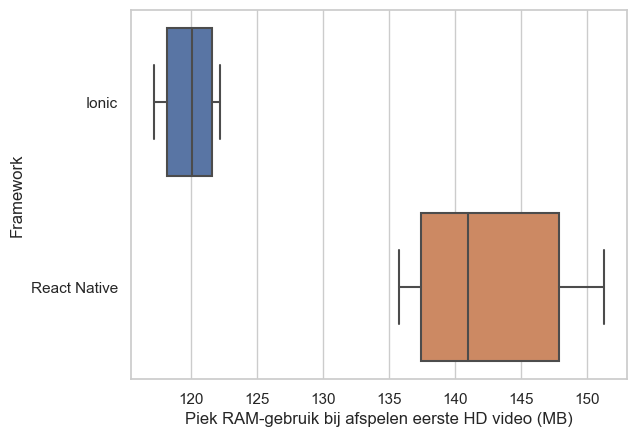
\includegraphics[width=0.7\linewidth]{img/ram/HD1}
  \caption{Boxplot van het piek-geheugengebruik van Ionic en React Native applicaties bij het afspelen van de eerste 1080p video}
  \label{fig:Boxplot van het piek-geheugengebruik van Ionic en React Native applicaties bij het afspelen van de eerste 1080p video}
\end{figure}

\begin{figure}
  \centering
  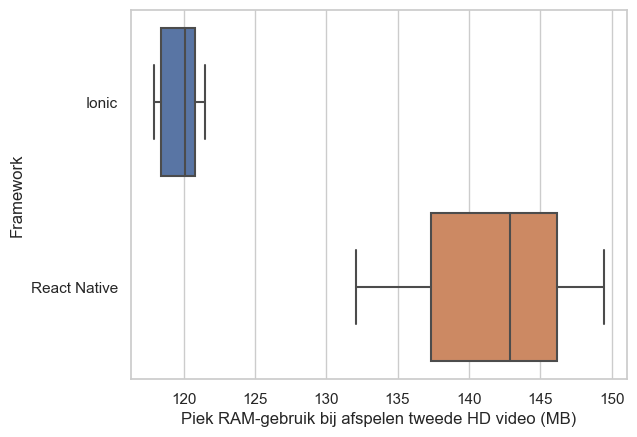
\includegraphics[width=0.7\linewidth]{img/ram/HD2}
  \caption{Boxplot van het piek-geheugengebruik van Ionic en React Native applicaties bij het afspelen van de tweede 1080p video}
  \label{fig:Boxplot van het piek-geheugengebruik van Ionic en React Native applicaties bij het afspelen van de tweede 1080p video}
\end{figure}

\begin{figure}
  \centering
  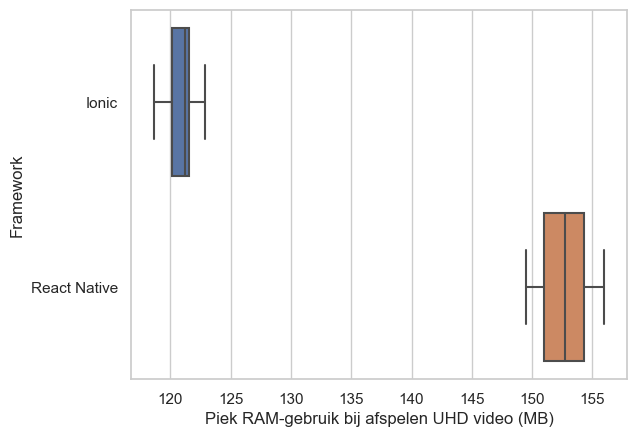
\includegraphics[width=0.7\linewidth]{img/ram/4k}
  \caption{Boxplot van het piek-geheugengebruik van Ionic en React Native applicaties bij het afspelen van de 4k video}
  \label{fig:Boxplot van het piek-geheugengebruik van Ionic en React Native applicaties bij het afspelen van de 4k video}
\end{figure}

TEKSTTTT

\begin{table}[htbp]
  \centering
  \footnotesize
  \begin{tabular}{|c|c|c|}
      \hline
      \textbf{Scenario} & \textbf{P-waarde} & \textbf{Beste resultaat} \\
      \hline
      Na opstarten & \(0.00046\) & Ionic \\
      \hline
      Eerste HD-video & \(1.371^{-11}\) & Ionic \\
      \hline
      Tweede HD-video & \(1.807^{-10}\) & Ionic \\
      \hline
      UHD-video & \(7.690^{-25}\) & Ionic \\
      \hline
  \end{tabular}
  \caption{Resultaten van de t-test voor het CPU-gebruik bij het afspelen van video's}
  \label{tab:cpu_ttest}
\end{table}

+++TEKSTTT


\subsection{Groottes van de applicaties}
\label{subsec:groottes-van-de-applicaties}

In dit laatste onderdeel zal er nog even kort stilgestaan worden bij de groottes van de APK-bestanden. Dit heeft niet noodzakelijk een impact op de performantie, maar toont wel 

(nog uit te schrijven)
%Wanneer we kijken naar de omvang van de APK-bestanden voor React en Ionic, zien we een aanzienlijk verschil. De APK-bestandsgrootte voor React bedraagt 155 MB, terwijl die voor Ionic slechts 3,76 MB is. Dit enorme verschil in bestandsgrootte kan verschillende oorzaken hebben, waaronder de complexiteit van de frameworks, de gebruikte bibliotheken en de manier waarop de applicaties worden gebouwd. Over het algemeen suggereert dit dat Ionic mogelijk lichtere en meer efficiënte APK-bestanden produceert in vergelijking met React, wat belangrijk kan zijn voor gebruikers met beperkte opslagruimte op hun apparaten of voor situaties waarin snelle download- en installatietijden van de applicatie van belang zijn.

React Native:
  - 155 MB .apk size

Ionic: 
  - 3.76 MB .apk size

(zeer opvallende situatie maar heeft waarschijnlijk te maken met het feit dat React Native de componenten in de app zelf moet inladen, terwijl Ionic gebruik maakt van de webview-engine van het toestel)

% Voeg hier je eigen hoofdstukken toe die de ``corpus'' van je bachelorproef
% vormen. De structuur en titels hangen af van je eigen onderzoek. Je kan bv.
% elke fase in je onderzoek in een apart hoofdstuk bespreken.

%\input{...}
%\input{...}
%...

%%=============================================================================
%% Conclusie
%%=============================================================================

\chapter{Conclusie}%
\label{ch:conclusie}

% TODO: Trek een duidelijke conclusie, in de vorm van een antwoord op de
% onderzoeksvra(a)g(en). Wat was jouw bijdrage aan het onderzoeksdomein en
% hoe biedt dit meerwaarde aan het vakgebied/doelgroep? 
% Reflecteer kritisch over het resultaat. In Engelse teksten wordt deze sectie
% ``Discussion'' genoemd. Had je deze uitkomst verwacht? Zijn er zaken die nog
% niet duidelijk zijn?
% Heeft het onderzoek geleid tot nieuwe vragen die uitnodigen tot verder 
%onderzoek?

Met de Proof-of-Concept kon er een duidelijk en uitgebreid beeld geschetst worden van de verschillen tussen React Native en Ionic omtrent streaming en de impact op de performantie. Het is nu belangrijk de bevindingen hier te bespreken en een verklaring te bieden voor de verschijnselen die zich voordeden. Tot slot zal er ook nog een aanleg gegeven worden voor toekomstig onderzoek binnen dit domein en nog een kleine reflectie gegeven worden.

\section{Verklaringen}
\label{sec:verklaringen}

Een eerste aspect dat werd onderzocht, waren de laadtijden van de applicaties. Zowel de cold als de warm startup-tijden werden hierbij gemeten. Het grootste verschil was op te merken bij de initiële opstart, waarbij Ionic een zeer grote voorsprong had op React Native met een verschil van minimum 3 seconden. De verklaring hiervoor is dat Ionic namelijk enkel en alleen, in het geval van de streaming-applicatie, het WebView-component moest raadplegen. React Native daarentegen maakt gebruik van verschillende andere componenten van het Android OS en moet bijgevolg meer tijd spenderen aan het inladen en renderen van deze componenten. De warm startup-tijden waren dan weer vrij gelijkaardig. Hoewel React Native een kleine voorsprong had, ging dit slechts over enkele milliseconden en is dit verschil vrijwel verwaarloosbaar. Dit valt dan weer te verklaren doordat de applicatie reeds opgestart is en de componenten reeds in het geheugen ingeladen zijn.

Een volgend onderdeel uit de Proof-of-Concept, was de interactie met de app. Hierbij bleek het verschil opnieuw te gaan over enkele honderden milliseconden. Ionic kwam net iets beter uit de resultaten dan React Native. Dit valt opnieuw te verklaren door het feit dat React Native met meer native componenten moet werken, waardoor er een kleine vertraging optreedt. Ondanks dat dit over enkele milliseconden gaat, kan dit toch een effect hebben op de gebruikerservaring. Indien een gebruiker snel zou willen wisselen tussen de video's, kan dit kleine verschil toch na een tijdje beginnen oplopen, waardoor er niet langer over milliseconden gesproken moet worden, maar eerder over seconden. Beide applicaties scoorden echter even goed op het effectieve streamen van de video's. De haperingen die optraden of het geluid dat niet altijd even synchroon met het beeld was, waren eerder te wijten aan de emulator zelf, dan aan de applicaties. Dit vanwege het feit dat deze vertragingen ook aanwezig waren bij het scrollen tussen de applicaties van het toestel en bij het navigeren op het web.

Het CPU-gebruik kan verdeeld worden in twee groepen op basis van de resultaten: het opstarten van de applicatie en het streamen van een video. Bij het opstarten bleek React Native de betere oplossing te zijn. Ionic moet namelijk bij de initiële opstart de code eerst nog compilen in de WebView, waardoor er een iets hogere piek in het CPU-gebruik optreedt. React Native daarentegen heeft deze stap in mindere mate nodig omdat deze rechtstreeks communiceert met de View-elementen van het OS zelf. Het streamen zelf verliep dan weer iets beter bij Ionic. Dit valt te verklaren omdat de WebView bij Ionic geoptimaliseerd is om videobestanden af te spelen en om te gaan met andere multimedia. React Native moet opnieuw met de verschillende OS-componenten communiceren, en vanwege de Fabric-architectuur die React Native hanteert, waarbij er zowel met JavaScript als met C++ gecommuniceerd wordt om de componenten te renderen, kan dit een verklaring zijn voor het hogere CPU-gebruik. Daarnaast had de hogere videoresolutie ook een invloed op het CPU-gebruik. Hoe hoger de resolutie, hoe meer rekenkracht er nodig is om de video af te spelen.

Tot slot werd er ook nog gekeken naar het geheugengebruik van beide applicaties. Eens de applicatie was opgestart leek het verschil aanvankelijk nog vrij miniem, maar toen de video begon te streamen, werd het verschil al snel duidelijk. React Native had een veel hoger geheugengebruik dan Ionic. Ook hier kan dezelfde verklaring worden gegeven als bij het CPU-gebruik. React Native moet met verschillende componenten van het OS communiceren die ingeladen zijn in het geheugen. Bovendien zorgt het gebruik van de Fabric-architectuur ervoor dat er meer complexe data onthouden moet worden om de componenten te renderen, hoe de video te decoden en natuurlijk af te spelen.

Er kan dus besloten worden dat over het algemeen Ionic beter scoorde dan React Native. Dit kan misschien zelf gezien worden als een eerder onverwacht resultaat voor sommigen, omdat uit verschillende bronnen vaak wordt beweerd dat Cross-Platform frameworks een performantie-voordeel hebben ten opzichte van Hybrid frameworks door het gebruik van native componenten. Deze mindset lijkt nog sterk ingeburgerd te zijn ondanks dat deze beweringen vaak op basis waren van onderzoeken die al lang achterhaald zijn. Het is dus belangrijk om steeds de nieuwste technologieën te onderzoeken en te vergelijken met elkaar om zo een correct beeld te krijgen van de huidige stand van zaken.

\section{Toekomstig onderzoek}
\label{sec:toekomstig-onderzoek}

De Proof-of-Concept heeft een duidelijk beeld geschetst van de verschillen tussen React Native en Ionic omtrent streaming. Toch zijn er nog enkele zaken die verder onderzocht kunnen worden naar de toekomst toe. Zo werd er voor dit onderzoek specifiek gekeken naar het Ionic-framework omdat deze toelaat om naast het gebruik van webtechnologieën ook gebruik te maken van native componenten van het OS zelf, zoals bijvoorbeeld de GPS of de camera. Hier werd er echter niet dieper op ingegaan. Het zou bijvoorbeeld interessant kunnen zijn om te onderzoeken hoe Ionic precies omgaat met deze native componenten en welke impact dit heeft op de performantie van de applicatie. Dit kan dan opnieuw vergeleken worden met React Native of eventueel een ander Cross-Platform framework om zo ook het native-aspect te vergelijken tussen Hybrid en Cross-Platform frameworks.


\section{Korte reflectie}
\label{sec:korte-reflectie}

Het principe dat er altijd native ontwikkeld moet worden voor de beste performantie, lijkt nog iets te zijn dat sterk ingeburgerd is in de ontwikkelingswereld. Desondanks kampen IT-bedrijven of programmeurs soms met een beperkt budget om een applicatie meermaals te implementeren op verschillende platformen. Dit onderzoek was dan ook vooral voor hen bedoeld om een duidelijk beeld te schetsen van de verschillen tussen Cross-Platform en Hybrid frameworks. Hoewel de keuze van het framework afhankelijk is van de noden van de applicatie, kan er toch besloten worden dat Ionic op vlak van prestaties beter scoort dan React Native als het gaat over streaming. Dit kan dan ook een belangrijke factor zijn bij het maken van een keuze voor een framework. Daarnaast valt wel op te merken dat Ionic nog vooral steunt op hun eigen community om native functionaliteiten te implementeren, terwijl React Native hier al een stuk verder in staat. De keuze van het framework zal dus vooral afhangen van de noden van de applicatie en wat het te bereiken doel is.

%---------- Bijlagen -----------------------------------------------------------

\appendix

\chapter{Onderzoeksvoorstel}

Het onderwerp van deze bachelorproef is gebaseerd op een onderzoeksvoorstel dat vooraf werd beoordeeld door de promotor. Dat voorstel is opgenomen in deze bijlage.

%% TODO: 
%\section*{Samenvatting}

% Kopieer en plak hier de samenvatting (abstract) van je onderzoeksvoorstel.

% Verwijzing naar het bestand met de inhoud van het onderzoeksvoorstel
%---------- Inleiding ---------------------------------------------------------

\section{Introductie}%
\label{sec:introductie}

Op vlak van mobiele app-ontwikkeling is er altijd een tweestrijd tussen het ontwikkelen voor Android en/of iOS. Het ontwikkelen voor beide platformen op een Native-aanpak voor dezelfde applicatie is echter een kostelijke en tijdrovende onderneming. De meeste Android applicaties worden geschreven met een combinatie van Java en Kotlin, terwijl iOS applicaties geschreven zijn in de door Apple ontwikkelde programmeertaal Swift. Het Native programmeren, d.w.z. het ontwikkelen van een applicatie specifiek bedoeld om te draaien op een bepaald platform, zorgt ervoor dat Swift-applicaties niet kunnen draaien op Android-platformen en omgekeerd. Vandaar het kostelijke aspect van het ontwikkelen voor beide platformen.

Cross-platform ontwikkelen biedt een oplossing voor dit probleem. De applicatie wordt hierbij één keer geschreven en kan vervolgens op verschillende platformen draaien. Dit wordt dan geprogrammeerd in talen die op verschillende platformen kunnen draaien zoals bijvoorbeeld JavaScript en C#. Hierbij is het grote nadeel dat de applicatie niet volledig is geoptimaliseerd voor het platform waarop het draait. Dit kan zelf leiden tot een tragere applicatie en een slechtere gebruikerservaring.

Dit bachelorproef zal zich focussen op het vergelijken van twee cross-platform frameworks, namelijk React Native en Ionic, op het Android-platform. React Native is een framework dat ontwikkeld is door Facebook en Ionic een framework dat ontwikkeld is door Drifty Co. Bij deze vergelijking zal er specifiek gekeken worden naar de performantie van de applicaties op basis van CPU-verbruik, laadtijden en geheugengebruik. De keuze voor deze specifieke frameworks is gebaseerd op de populariteit van deze frameworks, aangezien deze twee van de meest gebruikte cross-platform frameworks zijn.  Beide frameworks zijn bovendien open-source en gratis te gebruiken, wat de toegankelijkheid juist vergroot.

Hiervoor zal er een Proof-of-Concept worden uitgevoerd waarbij er een identieke applicatie zal worden ontwikkeld in React Native en Ionic. Deze applicaties zullen vervolgens getest worden op eerder vermelde performantie-aspecten. De resultaten van deze testen zullen tot slot worden geanalyseerd en vergeleken. Er zullen verschillende versies van deze applicaties worden ontwikkeld. Dit om uitvoerig en diepgaand te testen welke aspecten in welk framework een hogere impact hebben op de performantie. Zo kan er een uitgebreid beeld worden geschetst wat de voor- en nadelen zijn van beide frameworks.

Het onderzoek is gericht op ontwikkelaars en kleinere of middelgrote organisaties die met een beperkt budget hun applicatie op een zo groot mogelijke markt willen uitbrengen. Het onderzoek zal een antwoord bieden op de vraag welk framework het meest geschikt is voor het ontwikkelen van een performante applicatie op het Android-platform. Dit zal een meerwaarde bieden voor deze doelgroep, aangezien zij op basis van dit onderzoek een weloverwogen keuze kunnen maken voor het ontwikkelen van hun applicatie.


%---------- Stand van zaken ---------------------------------------------------

\section{State-of-the-art}%
\label{sec:state-of-the-art}

\paragraph{Native vs Cross-Platform}
\newline
Allereerst is het belangrijk om het verschil tussen native en cross-platform applicaties te omkaderen. Zoals eerder vermeld, verwijst Native programmeren naar het ontwikkelen van een applicatie bedoeld om te draaien op een gekozen platform. Dit betekent dat de applicatie geschreven is in de programmeertaal die specifiek bedoeld is voor het platform waarop het draait. Denk maar bijvoorbeeld aan Java en Kotlin voor Android. Cross-platformen daarentegen maken gebruik van onafhankelijke frameworks en talen die op verschillende platformen kunnen draaien (bv JavaScript). Deze worden vervolgens omgezet naar Native code en Native componenten specifiek aan het platform waarop het draait (BRON2).

Een voorbeeld van een Cross-Platform applicatie is een Hybride applicatie. Hierbij wordt er gesteund op webtechnologieën zoals HTML, CSS en JavaScript. Deze applicatie draait vervolgens in een native container van het specifieke platform. Dit wil zeggen dat de applicatie in de browser-engine van het desbetreffende platform draait (bron6). Bij Android is dit het WebView component, bij iOS wordt het UIWebView component gebruikt (BRON4). Aan de hand van een abstractielaag wordt er vervolgens toegang verkregen tot de mogelijkheden van het apparaat via JavaScript-API's (Bron6). Deze abstractielaag kan echter wel voor tragere prestaties zorgen, vooral op de CPU, aangezien de applicatie niet volledig "Native" is en als gevolg niet volledig geoptimaliseerd is aan het platform++++(Bron1).

\paragraph{React Native vs Ionic}
\newline
Voor dit onderzoek is er specifiek gekozen voor React Native en Ionic. Beide zijn cross-platform frameworks die gebruik maken van JavaScript als basis. Ionic is een open-source Hybrid framework ontwikkeld door Drifty Co? en laat toe om te werken met populaire JavaScript frameworks zoals Angular, React en Vue(https://ionicframework.com/docs#license).+++++ (2019 rework) (++++++ hoe weergeven??????)+++++++++++++++++++
React Native is, net zoals Ionic, een open-source framework. Het is ontwikkeld door Facebook en laat toe om te werken met React(bron3). Uit het brononderzoek bleek al snel dat er een paar misconcepties zijn over React Native. Zo wordt het vaak verkeerd beschouwd als een volledig "Native" framework. Het is en blijft Hybrid door het gebruik van JavaScript en JSX (een extensie van JavaScript) componenten. Het "Native" aspect in de naam verwijst naar het feit dat het framework gebruik maakt van Native UI-elementen (bron2). De JSX-componenten worden als het ware omgezet naar Native UI-elementen. Vandaar dat dit soms verkeerd wordt gecategoriseerd.
VM???????????????????????
SAMENVATTENDE ZIN

\paragraph{Architectuur van Android}
\newline
https://developer.android.com/guide/platform

IMAGE
++++++++++++
Het Android platform is een mobiele architectuur ontwikkeld door Google. Deze wordt opgedeeld in de volgende lagen:
  - System Apps: Dit zijn een verzameling standaardapplicaties die worden meegeleverd met het Android-platform. ++++ email sms etc 
  - Java API Framework: Deze laag biedt een set van functionaliteiten die gebruikt worden door +++++
  - Native C/C++ Libraries: Hierin bevinden zich de kerncomponenten en services van Android geschreven in C en C++ code. Daarnaast bevat dit ook de Java OpenGL API die instaat voor het renderen van 2D en 3D graphics.
  - Android Runtime (ART): Dit is de virtuele machine van Android doe de applicaties uitvoert. Enkele features van ART zijn onder andere garbage collection, just-in-time (JIT) compilatie en ahead-of-time (AOT) compilatie.
  - Hardware Abstraction Layer (HAL): Deze laag biedt een interface naar de onderliggende hardware. Deze zorgt ervoor dat de bovenliggende lagen niet rechtstreeks moeten communiceren met de hardware. Het bestaat uit verschillende library modules die elk een specifiek hardwarecomponent vertegenwoordigen.
  - Linux Kernel: Ook wel de kern van het Android-platform. Deze biedt een hardware-abstractielaag, een beveiligingsmodel, process management, geheugen management en een netwerkstack. Daarnaast biedt het ook drivers voor de verschillende hardwarecomponenten+++++.



%Dit state-of-the-art overzicht biedt een basis voor verder onderzoek naar de prestatieoptimalisatie van mobiele apps met specifieke aandacht voor React Native en Ionic op het Android-platform.


%Hier beschrijf je de \emph{state-of-the-art} rondom je gekozen onderzoeksdomein, d.w.z.\ een inleidende, doorlopende tekst over het onderzoeksdomein van je bachelorproef. Je steunt daarbij heel sterk op de professionele \emph{vakliteratuur}, en niet zozeer op populariserende teksten voor een breed publiek. Wat is de huidige stand van zaken in dit domein, en wat zijn nog eventuele open vragen (die misschien de aanleiding waren tot je onderzoeksvraag!)?

%Je mag de titel van deze sectie ook aanpassen (literatuurstudie, stand van zaken, enz.). Zijn er al gelijkaardige onderzoeken gevoerd? Wat concluderen ze? Wat is het verschil met jouw onderzoek?

%Verwijs bij elke introductie van een term of bewering over het domein naar de vakliteratuur, bijvoorbeeld~\autocite{Hykes2013}! Denk zeker goed na welke werken je refereert en waarom.

%Draag zorg voor correcte literatuurverwijzingen! Een bronvermelding hoort thuis \emph{binnen} de zin waar je je op die bron baseert, dus niet er buiten! Maak meteen een verwijzing als je gebruik maakt van een bron. Doe dit dus \emph{niet} aan het einde van een lange paragraaf. Baseer nooit teveel aansluitende tekst op eenzelfde bron.

%Als je informatie over bronnen verzamelt in JabRef, zorg er dan voor dat alle nodige info aanwezig is om de bron terug te vinden (zoals uitvoerig besproken in de lessen Research Methods).

% Voor literatuurverwijzingen zijn er twee belangrijke commando's:
% \autocite{KEY} => (Auteur, jaartal) Gebruik dit als de naam van de auteur
%   geen onderdeel is van de zin.
% \textcite{KEY} => Auteur (jaartal)  Gebruik dit als de auteursnaam wel een
%   functie heeft in de zin (bv. ``Uit onderzoek door Doll & Hill (1954) bleek
%   ...'')

Je mag deze sectie nog verder onderverdelen in subsecties als dit de structuur van de tekst kan verduidelijken.

%---------- Methodologie ------------------------------------------------------
\section{Methodologie}%
\label{sec:methodologie}

Hier beschrijf je hoe je van plan bent het onderzoek te voeren. Welke onderzoekstechniek ga je toepassen om elk van je onderzoeksvragen te beantwoorden? Gebruik je hiervoor literatuurstudie, interviews met belanghebbenden (bv.~voor requirements-analyse), experimenten, simulaties, vergelijkende studie, risico-analyse, PoC, \ldots?

Valt je onderwerp onder één van de typische soorten bachelorproeven die besproken zijn in de lessen Research Methods (bv.\ vergelijkende studie of risico-analyse)? Zorg er dan ook voor dat we duidelijk de verschillende stappen terug vinden die we verwachten in dit soort onderzoek!

Vermijd onderzoekstechnieken die geen objectieve, meetbare resultaten kunnen opleveren. Enquêtes, bijvoorbeeld, zijn voor een bachelorproef informatica meestal \textbf{niet geschikt}. De antwoorden zijn eerder meningen dan feiten en in de praktijk blijkt het ook bijzonder moeilijk om voldoende respondenten te vinden. Studenten die een enquête willen voeren, hebben meestal ook geen goede definitie van de populatie, waardoor ook niet kan aangetoond worden dat eventuele resultaten representatief zijn.

Uit dit onderdeel moet duidelijk naar voor komen dat je bachelorproef ook technisch voldoen\-de diepgang zal bevatten. Het zou niet kloppen als een bachelorproef informatica ook door bv.\ een student marketing zou kunnen uitgevoerd worden.

Je beschrijft ook al welke tools (hardware, software, diensten, \ldots) je denkt hiervoor te gebruiken of te ontwikkelen.

Probeer ook een tijdschatting te maken. Hoe lang zal je met elke fase van je onderzoek bezig zijn en wat zijn de concrete \emph{deliverables} in elke fase?

%---------- Verwachte resultaten ----------------------------------------------
\section{Verwacht resultaat, conclusie}%
\label{sec:verwachte_resultaten}

Hier beschrijf je welke resultaten je verwacht. Als je metingen en simulaties uitvoert, kan je hier al mock-ups maken van de grafieken samen met de verwachte conclusies. Benoem zeker al je assen en de onderdelen van de grafiek die je gaat gebruiken. Dit zorgt ervoor dat je concreet weet welk soort data je moet verzamelen en hoe je die moet meten.

Wat heeft de doelgroep van je onderzoek aan het resultaat? Op welke manier zorgt jouw bachelorproef voor een meerwaarde?

Hier beschrijf je wat je verwacht uit je onderzoek, met de motivatie waarom. Het is \textbf{niet} erg indien uit je onderzoek andere resultaten en conclusies vloeien dan dat je hier beschrijft: het is dan juist interessant om te onderzoeken waarom jouw hypothesen niet overeenkomen met de resultaten.



%%---------- Andere bijlagen --------------------------------------------------
% TODO: Voeg hier eventuele andere bijlagen toe. Bv. als je deze BP voor de
% tweede keer indient, een overzicht van de verbeteringen t.o.v. het origineel.
%\input{...}

%%---------- Backmatter, referentielijst ---------------------------------------

\backmatter{}

\setlength\bibitemsep{2pt} %% Add Some space between the bibliograpy entries
\printbibliography[heading=bibintoc]

\end{document}
